\section{Quantum Quasi Particles and the Quantum Pinball Propagator}
In the quantum case, the total probability amplitude is the sum of the probability amplitudes for each process taken separately
$$G(2,1)=G(\text { process } 1)+G(\text { process } 11)+\cdots$$
so that the corresponding probability is given by
$$P(2,1)_{\text {quantum }}=G^{*} G=\underbrace{|G(\mathrm{I})|^{2}}_{P(\mathrm{I})}+\underbrace{|G(\mathrm{I})|^{2}}_{P(\mathrm{II})}+\underbrace{G(\mathrm{I})^{*} G(\mathrm{II})+G(\mathrm{II})^{*} G(\mathrm{I})}_{\text {interference terms }}+\cdots$$
Because of the characteristic interference terms', the quantum probability is not just the sum of the probabilities for the individual processes, in contrast to the classical case.

Let us begin by defining the quantum propagator in general, then show
what it looks like in the case of free particles and quasi particles. The quantum analogue of the classical propagator is (assuming that the Hamiltonian is time-independent, so that the propagator depends only on time differences):
\begin{imp}
\begin{equation}i G\left(\mathrm{r}_{2}, \mathrm{r}_{1}, t_{2}-t_{1}\right)_{t_{2}>t_{1}}=i G^{+}\left(\mathrm{x}_{2}, \mathrm{r}_{1}, t_{2}-t_{1}\right)\end{equation}
probability amplitude that if at time $t_{1}$ we add a particle at point $r_{1}$ to the interacting system in its ground state, then at time $t_{2}$ the system will be in its ground state with an added particle at $\mathbf{r}_{2}$
\end{imp}
The $i$ factor is purely for decoration (a matter of convention) and the $+$ superscript denotes $t_{2}>t_{1} .$ The probability corresponding to the amplitude is
$$P\left(\mathbf{r}_{2}, \mathbf{r}_{1}, t_{2}-t_{1}\right)=G^{+}\left(r_{2}, \mathbf{r}_{1}, t_{2}-t_{1}\right)^{*} G^{+}\left(\mathbf{r}_{2}, \mathbf{r}_{1}, t_{2}-t_{1}\right)$$
Note that it is not necessarily the 'same' particle which is observed at 12, since
this has no meaning in the systems of identical particles with which we shall generally deal. The quantity $G^{+}$ is called a \bluep{'retarded' propagator (or Green's function)}. By definition, it is equal to zero for $t_{2} \leqslant t_{1} .$ There is also an \bluep{'advanced' propagator, $G^{-},$ which is finite for $t_{2} \leqslant t_{1} $}.

It is actually more convenient to work with an equivalent definition of $G$ in terms of arbitrary single-particle eigenstates, $\phi_{k}(r),$ instead of position eigenstates. Then we have \redp{$i G^{+}\left(k_{2}, k_{1}, t_{2}-t_{1}\right)_{t_{2}>t_{1}}=$probability amplitude that if at time $t_{1}$ we add a particle in $\phi_{k_{1}}(r)$ to the interacting system in its ground state, then at time $t_{2}$ the system will be in its ground state with an added particle in $\phi_{k_{2}}(r)$}.
For $t_{2} \leqslant t_{1}, G^{+}$ is defined so that:
\begin{equation}i G^{+}\left(k_{2}, k_{1}, t_{2}-t_{1}\right)_{t_{2}\leq t_{1}}=0\end{equation}
\textbf{A convenient choice for $\phi_{k}(r)$ is the eigenstates of the unperturbed single particle Hamiltonian, which we will call $H_{0}$ :}
$$H_{0}=\frac{p^{2}}{2 m}+U(\mathrm{r})=-\frac{1}{2 m} \nabla_{r}^{2}+U(\mathrm{r}) \quad(\hbar=1)$$
If $U(\mathrm{r})=0,$ then this is just the free particle case:
$$H_{0} \phi_{k}(\mathbf{r})=\epsilon_{k} \phi_{k}(\mathbf{r})$$
and
\begin{equation}H_{0}=-\frac{\nabla_{r}^{2}}{2 m}, \quad \phi_{k}(r)=\frac{1}{\sqrt{\Omega}} e^{i k \cdot r}, \quad \epsilon_{k}=\frac{k^{2}}{2 m}
\label{nrqm-free-particle}
\end{equation}
where $\Omega$ is normalization volume and spin is neglected for simplicity. Note that if $k_1=k_2$, the particle propagates in time only.

Let us first get the free propagator $G_{0}^{+}$ (no perturbing interaction). Suppose at time $t_{1}$ the wave function of the free particle is $\phi_{k,}(\mathrm{r}) .$ Then we have:
$$\psi\left(\mathbf{r}, t_{1}\right)=\phi_{\mathbf{k}_{2}}(\mathbf{r})$$
At later time $t_{2},$ by the time-dependent Schrödinger equation, we find that the wave function has become
\begin{equation}\psi\left(\mathbf{r}, t_{2}\right)=\phi_{k_{1}}(\mathbf{r}) e^{-i \varepsilon_{k1}\left(t_{2}-t_{1}\right)}
\end{equation}
where $\epsilon_{k_{1}}$ is the single particle energy of undisturbed Shrodinger equation. The probability amplitude for the particle being in state $\phi_{k_{2}}$ at time $t_{2}$ is /hen just the component of $\psi\left(\mathbf{r}, t_{2}\right)$ along $\phi_{k_{2}}$ or:
\begin{equation}\int d^{3} \mathbf{r} \psi\left(\mathbf{r}, t_{2}\right) \phi_{k_{2}}^{*}(\mathbf{r})=e^{-i \exp \left(l_{2}-t_{1}\right)} \int \underbrace{d^{3} \mathbf{r} \phi_{k_{1}}(\mathbf{r}) \phi_{k_{2}}^{*}(\mathbf{r})}_{\delta_{k_{2} k_{1}}}\end{equation}
whence, by definition
\begin{equation}G_{0}^{+}\left(k, t_{2}-t_{1}\right)=\left\{\begin{array}{ll}
-i \theta_{12-t_{1}} e^{-i \epsilon_{k_1}\left(t_{2}-t_{1}\right)}, & \text { for } t_{2} \neq t_{1} \\
0, & \text { for } t_{2}=t_{1}
\end{array}\right.
\label{G0-+}
\end{equation}
where
$$\theta_{t_{2}-t_{1}}\left\{\begin{array}{ll}
=1, & \text { if } t_{2}>t_{1} \\
=0, & \text { if } t_{2}<t_{1}
\end{array}\right.$$
\bluep{Note that for fermions, all levles up to $\epsilon_F$(=Fermi energy) are fileed, so we can only propagate a particle with $\epsilon_{k_1}>\epsilon_F$}. The Fourier transform of (\ref{G0-+}) is
\begin{equation}\begin{aligned}
G_{0}^{+}(k, \omega) &=-i \int_{-\infty}^{+\infty} d\left(t_{2}-t_{1}\right) \theta_{t_{2}-t_{1}} e^{i \omega\left(t_{2}-t_{1}\right)} e^{-i \epsilon_{k}\left(t_{2}-t_{1}\right)} \\
&=\left.(-1) \frac{e^{i\left(\omega-\epsilon_{k}\right)\left(t_{2}-t_{1}\right)}}{\omega-\epsilon_{k}}\right|_{0} ^{\infty}=\frac{1}{\omega-\epsilon_{k}}-\frac{e^{i\left(\omega-\epsilon_{k}\right)\infty}}{\omega-\epsilon_{k}}
\end{aligned}
\label{G0-k-omega}
\end{equation}
\redp{Because of the exponential oscillating at $\infty,$ this function is not well defined. In order to get around this difficulty, we have to slightly modify the expression for the free propagator. This is done by multiplying the propagator by the factor $\exp \left(-\delta\left(t_{2}-t_{1}\right)\right),$ where $\delta$ is a positive infinitesimal such that $\delta \times \infty=\infty$}. Then (\ref{G0-+}) becomes:
\begin{equation}G_{0}^{+}\left(k, t_{2}-t_{1}\right)=-i \theta_{t_{2}-t_{1}}e^{i(\epsilon_k-i\delta)(t_2-t_1)}
\label{G0-with-delta}
\end{equation}
For any finite $\left(t_{2}-t_{1}\right),$ we have $\delta \times\left(t_{2}-t_{1}\right)=0,$ so this is just $(3.10) .$ But for infinite $\left(t_{2}-t_{1}\right), \delta \times\left(t_{2}-t_{1}\right)=\infty$ so $G_{0}^{+}=0 .$ When \ref{G0-with-delta} is placed in \ref{G0-k-omega} we find
\begin{imp}
\begin{equation}G_{o}^{+}(k, \omega)=\frac{1}{\omega-\epsilon_{k}+i \delta}
\label{G0-k-omega-delta}
\end{equation}
\end{imp}
\bluep{From \ref{G0-k-omega-delta} we see the pole is at $\omega=\epsilon_k$, the eigenvalue for the eigenstate $\phi_k$. It turns out this observation is quite general, even for interacting propagator, $G^+(k,l;\omega)$:}
\begin{imp}
The poles of $G^+(k,l,\omega),$ the fourier transform of the single-particle propagator, corresponds to the excited energy of (N+1)-particle system \textbf{minus the ground state energy of N-particle system}.
\end{imp}
Also from \ref{G0-k-omega-delta}, we have the particle lifetime $\tau$ as $\delta^{-1}=\infty$, which makes sense because we only consider one free particle here. This observation can also be extended to interacting system where the propagator has the form of 
\begin{equation}
    G^+=\frac{1}{\omega-\epsilon_k^{\prime}+i\tau_k^{-1}}
\end{equation}
where \redp{$\tau_k$ is the quasi-particle lifetime at the state of $\epsilon_k$}.

In a Fermi system, because of the Pauli's principle, each state can only be occupied by one fermion. If a state is partially occupied by a fermion, the possibility of adding another fermion at the same state will be less than 1. Hence we have to multiply the propagator by a factor $Z_k\leq 1$:
\begin{equation}G_{\text {\stackanchor{quasi}{particle} }}^{+}\left(k,t_{2}-t_{1}\right)=-i Z_{k} e^{-i \epsilon_{k}^{\prime}\left(t_{2}-t_{1}\right)} e^{-\left(t_{2}-t_{1}\right) / \tau_{k}}\end{equation}
\begin{equation}G_{\text {\stackanchor{quasi}{particle}}}^{+}(k, \omega)=\frac{Z_{k}}{\omega-\epsilon_{k}^{\prime}+i \tau_{k}^{-1}}\end{equation}
The poles in the equation above are 
\begin{equation}
    \omega = \epsilon_k^{\prime}-i\tau_k^{-1}
\end{equation}
We can still interpret these poles as the excited energy levels even though they are imaginary numbers. For free particles, we have eigenstates as:
$$
\psi_k(x)=\phi_k(x)e^{-i\epsilon_k t}
$$
When the weak interaction is turned on, the particle decays out of state "$k$", we have
$$
\psi_k(x)\approx\phi_k(x)e^{-i\epsilon_k^{\prime} t}e^{-t/\tau_k}=\phi_k(x)e^{-i(\epsilon_k^{\prime}-i\tau^{-1})t}
$$

\subsection{Quantum Pinball Game}
Like the classical pinball game, we now consider the quantum version of the game where \redp{the "scattering centers" are now "scattering fields/potentials"}. Let's assume that a perturbative potential that interacts with free particle has a form of:
\begin{equation}V(\mathbf{p})=V_{M}+V_{L}=M p^{2}+L p^{4}=-M \nabla_{r}^{2}+L \nabla_{r}^{4}\end{equation}
where $M \geqslant L$. By solving the Schrodinger equation we have the Hamiltonian as
$$
H = (\frac{1}{2m}+M+Lp^2)p^2
$$
with 
$$
\epsilon_k^{\prime}= (\frac{1}{2m}+M+Lk^2)k^2
$$
and $\phi_k(x)=\frac{1}{\sqrt{\Omega}}e^{-i\mathbf{k}\cdot\mathbf{r}}$.\bluep{Now let us solve for the eigenvalues in a propagator way.}

The simplest way the particle can propagate through the system is without interaction, which has a propability amplitude as $G^+(k,t_2-t_1)$. Another way is to enter in $\phi_{k_{1}}$ at time $t_{1},$ be scattered into state $\phi_{k_{2}}$ at time $t_{M}$ by the potential $V_{M},$ then continue freely in $\phi_{k_{2}}$ until time $t_{2} .$ The probability amplitude in this case is just the product of the probability amplitude for each independent process:
$$
G^+_0(k_1,t_M-t_1)V_MG^+_0(k_1,t_2-t_M)
$$
$V_M$ can be obtained from time-dependent perturbation theory as follows: Let $c_{l}$ be the probability amplitude that at time $t_{0}$ a system is in state $\phi_{l} .$ Then at later time, $t,$ the time rate of change of any particular $c_{l},$ say $c_{p},$ under the influence of perturbation $V$, is given by:
\begin{equation}\dot{c}_{p}(t)=-i \sum_{l} V_{p l} c_{l} e^{i\left(\epsilon_{p}-\epsilon_{l}\right)\left(t-t_{o}\right)}\end{equation}
where $V_{pl}$ is just the element of S matrix. Hence the probability amplitude per unit time that the system undergoes a transition from $\phi_{k_1}$ to $\phi_p=\phi_{k_2}$, at time $t_M$ is:
\begin{equation}\begin{aligned}
\dot{c}_{k_{2}}\left(t=t_{M}\right) &=-i V_{M_{k_2 k_1}}=-i \int d^{3} \mathbf{r} \phi_{k_{2}}^{*}(r) V_{M} \phi_{k_{1}}(r)=\\
&=+i M \int d^{3} \mathbf{r} \phi_{k_{2}}^{*} \nabla^{2} \phi_{k_{1}}=-i M k_{1}^{2} \delta_{k_{2} k_{1}}
\end{aligned}\end{equation}
Thus the probability amplitude for this first-order scattering is 
\begin{equation}
    \left[\text{\stackanchor{probability}{amplitude}}\right]_{t_1\rightarrow t_M\rightarrow t_2}=i \int_{-\infty}^{+\infty} d t_{M} G_{0}^{+}\left(\mathbf{k}_{1}, t_{M}-t_{1}\right) V_{M_{k_2k_1}} G_{0}^{+}\left(\mathbf{k}_{2}, t_{2}-t_{M}\right)
\end{equation}
Similarly for $V_L$, we have
$$-i V_{L_{k_1k_2}}=-i L k_{1}^{4} \delta_{k_{2} k_{1}}$$
which also conserves momentum. There are also second- and higher-order processes in which the particle collides with $V_{M}$ and $V_{L}$ any number of times. This gives us the series expansion for the propagator (set $\mathbf{k}_{1}=\mathbf{k}_{2}=\mathbf{k}$ because of conservation of momentum here), after cancelling the $i$ 's:
$$\begin{aligned}
G^{+}\left(\mathbf{k}, t_{2}-t_{1}\right)=G_{0}^{+} &\left(\mathbf{k}, t_{2}-t_{1}\right)+\int_{-\infty}^{+\infty} d t_{M} G_{0}^{+}\left(\mathbf{k}, t_{M}-t_{1}\right) V_{M} G_{0}^{+}\left(\mathbf{k}, t_{2}-t_{M}\right) \\
&+\int_{-\infty}^{+\infty} d t_{L} G_{0}^{+}\left(\mathbf{k}, t_{L}-t_{1}\right) V_{L} G_{0}^{+}\left(\mathbf{k}, t_{2}-t_{L}\right)+\\
&+\int d t_{M} d t_{M}^{\prime} \cdots+\int d t_{M} d t_{L} \cdots+\cdots
\end{aligned}$$
Taking the Fourier transform, we have
\begin{equation}\begin{aligned}
G^{+}(\mathbf{k}, \omega)=G_{0}^{+} &(\mathbf{k}, \omega)+\left[G_{0}^{+}(\mathbf{k}, \omega)\right]^{2} V_{M_{k k}}+\left[G_{0}^{+}(\mathbf{k}, \omega)\right]^{2} V_{L_{kk}}+\\
&+\left[G_{0}^{+}\right]^{3} V_{M_{kk}}^{2}+2\left[G_{0}^{+}\right]^{3} V_{M_{kk}} V_{L_{kk}}+\left[G_{0}^{+}\right]^{3} V_{L_{kk}}^{2}+\\
&+\left[G_{0}^{+}\right]^{4} V_{M_{kk}}^{3}+\cdots
\end{aligned}\end{equation}
We now pull the trick of \redp{partial summation} here. We assume that the scattering with $V_M$ is much more important than the scattering with $V_L$, then the Feynman diagram series can be approximated by:
\begin{figure}[H]
    \centering
    


\tikzset{every picture/.style={line width=0.75pt}} %set default line width to 0.75pt        

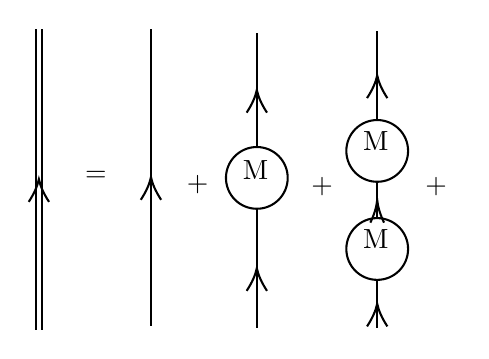
\begin{tikzpicture}[x=0.75pt,y=0.75pt,yscale=-1,xscale=1]
%uncomment if require: \path (0,300); %set diagram left start at 0, and has height of 300

%Straight Lines [id:da6679599183950475] 
\draw    (52.75,218.9) -- (52.75,73.9)(55.75,218.9) -- (55.75,73.9) ;
\draw [shift={(54.25,146.4)}, rotate = 450] [color={rgb, 255:red, 0; green, 0; blue, 0 }  ][line width=0.75]    (10.93,-4.9) .. controls (6.95,-2.3) and (3.31,-0.67) .. (0,0) .. controls (3.31,0.67) and (6.95,2.3) .. (10.93,4.9)   ;
%Straight Lines [id:da03187978212104414] 
\draw    (159.25,130.9) -- (159.25,75.9) ;
\draw [shift={(159.25,103.4)}, rotate = 450] [color={rgb, 255:red, 0; green, 0; blue, 0 }  ][line width=0.75]    (10.93,-4.9) .. controls (6.95,-2.3) and (3.31,-0.67) .. (0,0) .. controls (3.31,0.67) and (6.95,2.3) .. (10.93,4.9)   ;
%Shape: Circle [id:dp6720254680854465] 
\draw   (144.38,145.77) .. controls (144.38,137.56) and (151.03,130.9) .. (159.25,130.9) .. controls (167.47,130.9) and (174.13,137.56) .. (174.13,145.77) .. controls (174.13,153.99) and (167.47,160.65) .. (159.25,160.65) .. controls (151.03,160.65) and (144.38,153.99) .. (144.38,145.77) -- cycle ;
%Straight Lines [id:da38078856367120306] 
\draw    (159.25,160.65) -- (159.25,217.9) ;
\draw [shift={(159.25,189.27)}, rotate = 90] [color={rgb, 255:red, 0; green, 0; blue, 0 }  ][line width=0.75]    (10.93,-4.9) .. controls (6.95,-2.3) and (3.31,-0.67) .. (0,0) .. controls (3.31,0.67) and (6.95,2.3) .. (10.93,4.9)   ;
%Straight Lines [id:da45284041242528794] 
\draw    (108.25,216.9) -- (108.25,73.9) ;
\draw [shift={(108.25,145.4)}, rotate = 450] [color={rgb, 255:red, 0; green, 0; blue, 0 }  ][line width=0.75]    (10.93,-4.9) .. controls (6.95,-2.3) and (3.31,-0.67) .. (0,0) .. controls (3.31,0.67) and (6.95,2.3) .. (10.93,4.9)   ;
%Straight Lines [id:da05583872838111581] 
\draw    (217.25,117.9) -- (217.25,74.9) ;
\draw [shift={(217.25,96.4)}, rotate = 450] [color={rgb, 255:red, 0; green, 0; blue, 0 }  ][line width=0.75]    (10.93,-4.9) .. controls (6.95,-2.3) and (3.31,-0.67) .. (0,0) .. controls (3.31,0.67) and (6.95,2.3) .. (10.93,4.9)   ;
%Shape: Circle [id:dp6854080468003328] 
\draw   (202.38,132.77) .. controls (202.38,124.56) and (209.03,117.9) .. (217.25,117.9) .. controls (225.47,117.9) and (232.13,124.56) .. (232.13,132.77) .. controls (232.13,140.99) and (225.47,147.65) .. (217.25,147.65) .. controls (209.03,147.65) and (202.38,140.99) .. (202.38,132.77) -- cycle ;
%Shape: Circle [id:dp32578384863224485] 
\draw   (202.38,180.02) .. controls (202.38,171.81) and (209.03,165.15) .. (217.25,165.15) .. controls (225.47,165.15) and (232.13,171.81) .. (232.13,180.02) .. controls (232.13,188.24) and (225.47,194.9) .. (217.25,194.9) .. controls (209.03,194.9) and (202.38,188.24) .. (202.38,180.02) -- cycle ;
%Straight Lines [id:da6105349842531441] 
\draw    (217.25,165.15) -- (217.25,147.65) ;
\draw [shift={(217.25,156.4)}, rotate = 450] [color={rgb, 255:red, 0; green, 0; blue, 0 }  ][line width=0.75]    (10.93,-3.29) .. controls (6.95,-1.4) and (3.31,-0.3) .. (0,0) .. controls (3.31,0.3) and (6.95,1.4) .. (10.93,3.29)   ;
%Straight Lines [id:da308062636403606] 
\draw    (217.25,217.9) -- (217.25,194.9) ;
\draw [shift={(217.25,206.4)}, rotate = 450] [color={rgb, 255:red, 0; green, 0; blue, 0 }  ][line width=0.75]    (10.93,-4.9) .. controls (6.95,-2.3) and (3.31,-0.67) .. (0,0) .. controls (3.31,0.67) and (6.95,2.3) .. (10.93,4.9)   ;

% Text Node
\draw (75,141) node [anchor=north west][inner sep=0.75pt]   [align=left] {=};
% Text Node
\draw (124,143) node [anchor=north west][inner sep=0.75pt]   [align=left] {+};
% Text Node
\draw (184,144) node [anchor=north west][inner sep=0.75pt]   [align=left] {+};
% Text Node
\draw (239,144) node [anchor=north west][inner sep=0.75pt]   [align=left] {+};
% Text Node
\draw (255,141) node [anchor=north west][inner sep=0.75pt]    {$\dotsc $};
% Text Node
\draw (151,136) node [anchor=north west][inner sep=0.75pt]   [align=left] {M};
% Text Node
\draw (209,169) node [anchor=north west][inner sep=0.75pt]   [align=left] {M};
% Text Node
\draw (209,122) node [anchor=north west][inner sep=0.75pt]   [align=left] {M};


\end{tikzpicture}

    \caption{Partial Summation of Quantum Pinball Game}
    \label{fig:partial-sum-quantum-pinball}
\end{figure}
Convert this series to equation we have:
\begin{equation}
\begin{aligned}
G^+(\mathbf{k},\omega)&\approx G^+_0(\mathbf{k},\omega)+[G_0^+(\mathbf{k},\omega)]^2V_{M_{kk}}+[G_0^+]^3V_{M_{kk}}^2+\ldots\\
&=G_0^+(1+G_0^+V_M+(G_0^+V_M)^2+\ldots)\\
&=\frac{G_0^+(\mathbf{k},\omega)}{1-G_0^+(\mathbf{k},\omega)V_{M_{kk}}}
\end{aligned}
\end{equation}
Of course we can reproduce this calculation by manipulating the Feynman diagram series:
\begin{figure}[H]
\centering
\tikzset{every picture/.style={line width=0.75pt}} %set default line width to 0.75pt        

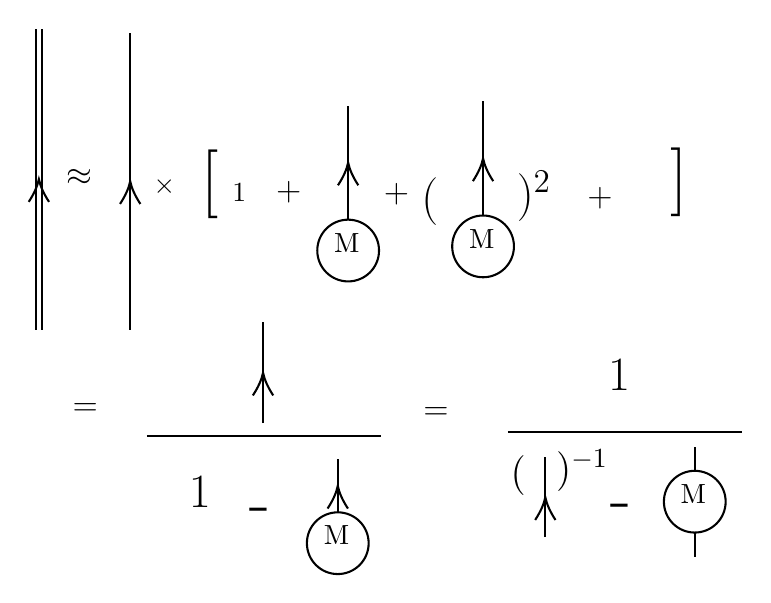
\begin{tikzpicture}[x=0.75pt,y=0.75pt,yscale=-1,xscale=1]
%uncomment if require: \path (0,300); %set diagram left start at 0, and has height of 300

%Straight Lines [id:da6679599183950475] 
\draw    (43.75,155.9) -- (43.75,10.9)(46.75,155.9) -- (46.75,10.9) ;
\draw [shift={(45.25,83.4)}, rotate = 450] [color={rgb, 255:red, 0; green, 0; blue, 0 }  ][line width=0.75]    (10.93,-4.9) .. controls (6.95,-2.3) and (3.31,-0.67) .. (0,0) .. controls (3.31,0.67) and (6.95,2.3) .. (10.93,4.9)   ;
%Straight Lines [id:da3819886351076084] 
\draw    (89.25,155.9) -- (89.25,12.9) ;
\draw [shift={(89.25,84.4)}, rotate = 450] [color={rgb, 255:red, 0; green, 0; blue, 0 }  ][line width=0.75]    (10.93,-4.9) .. controls (6.95,-2.3) and (3.31,-0.67) .. (0,0) .. controls (3.31,0.67) and (6.95,2.3) .. (10.93,4.9)   ;
%Straight Lines [id:da40404534625465094] 
\draw    (194.25,102.9) -- (194.25,47.9) ;
\draw [shift={(194.25,75.4)}, rotate = 450] [color={rgb, 255:red, 0; green, 0; blue, 0 }  ][line width=0.75]    (10.93,-4.9) .. controls (6.95,-2.3) and (3.31,-0.67) .. (0,0) .. controls (3.31,0.67) and (6.95,2.3) .. (10.93,4.9)   ;
%Shape: Circle [id:dp10590981200217242] 
\draw   (179.38,117.77) .. controls (179.38,109.56) and (186.03,102.9) .. (194.25,102.9) .. controls (202.47,102.9) and (209.13,109.56) .. (209.13,117.77) .. controls (209.13,125.99) and (202.47,132.65) .. (194.25,132.65) .. controls (186.03,132.65) and (179.38,125.99) .. (179.38,117.77) -- cycle ;
%Straight Lines [id:da2189214793166505] 
\draw    (259.25,100.9) -- (259.25,45.9) ;
\draw [shift={(259.25,73.4)}, rotate = 450] [color={rgb, 255:red, 0; green, 0; blue, 0 }  ][line width=0.75]    (10.93,-4.9) .. controls (6.95,-2.3) and (3.31,-0.67) .. (0,0) .. controls (3.31,0.67) and (6.95,2.3) .. (10.93,4.9)   ;
%Shape: Circle [id:dp9920078778157783] 
\draw   (244.38,115.77) .. controls (244.38,107.56) and (251.03,100.9) .. (259.25,100.9) .. controls (267.47,100.9) and (274.13,107.56) .. (274.13,115.77) .. controls (274.13,123.99) and (267.47,130.65) .. (259.25,130.65) .. controls (251.03,130.65) and (244.38,123.99) .. (244.38,115.77) -- cycle ;
%Straight Lines [id:da44750961592695404] 
\draw    (189.25,243.9) -- (189.25,218.4) ;
\draw [shift={(189.25,231.15)}, rotate = 450] [color={rgb, 255:red, 0; green, 0; blue, 0 }  ][line width=0.75]    (10.93,-4.9) .. controls (6.95,-2.3) and (3.31,-0.67) .. (0,0) .. controls (3.31,0.67) and (6.95,2.3) .. (10.93,4.9)   ;
%Shape: Circle [id:dp036519837337342875] 
\draw   (174.38,258.77) .. controls (174.38,250.56) and (181.03,243.9) .. (189.25,243.9) .. controls (197.47,243.9) and (204.13,250.56) .. (204.13,258.77) .. controls (204.13,266.99) and (197.47,273.65) .. (189.25,273.65) .. controls (181.03,273.65) and (174.38,266.99) .. (174.38,258.77) -- cycle ;
%Straight Lines [id:da9791654199909201] 
\draw    (97.25,207.02) -- (210,207.02) ;
%Straight Lines [id:da49874010942747804] 
\draw    (153.25,200.9) -- (153.25,152.4) ;
\draw [shift={(153.25,176.65)}, rotate = 450] [color={rgb, 255:red, 0; green, 0; blue, 0 }  ][line width=0.75]    (10.93,-4.9) .. controls (6.95,-2.3) and (3.31,-0.67) .. (0,0) .. controls (3.31,0.67) and (6.95,2.3) .. (10.93,4.9)   ;
%Shape: Circle [id:dp7199868696958168] 
\draw   (346.38,238.77) .. controls (346.38,230.56) and (353.03,223.9) .. (361.25,223.9) .. controls (369.47,223.9) and (376.13,230.56) .. (376.13,238.77) .. controls (376.13,246.99) and (369.47,253.65) .. (361.25,253.65) .. controls (353.03,253.65) and (346.38,246.99) .. (346.38,238.77) -- cycle ;
%Straight Lines [id:da37789491773642436] 
\draw    (271.25,205.02) -- (384,205.02) ;
%Straight Lines [id:da3979415686562028] 
\draw    (289.25,255.9) -- (289.25,217.4) ;
\draw [shift={(289.25,236.65)}, rotate = 450] [color={rgb, 255:red, 0; green, 0; blue, 0 }  ][line width=0.75]    (10.93,-4.9) .. controls (6.95,-2.3) and (3.31,-0.67) .. (0,0) .. controls (3.31,0.67) and (6.95,2.3) .. (10.93,4.9)   ;
%Straight Lines [id:da6305145122698304] 
\draw    (361.25,223.9) -- (361.25,212.4) ;
%Straight Lines [id:da6086382662478782] 
\draw    (361.25,253.65) -- (361.25,265.4) ;

% Text Node
\draw (57,77.02) node [anchor=north west][inner sep=0.75pt]  [font=\large]  {$\approx $};
% Text Node
\draw (99,81.02) node [anchor=north west][inner sep=0.75pt]    {$\times $};
% Text Node
\draw (158,83) node [anchor=north west][inner sep=0.75pt]  [font=\large] [align=left] {+};
% Text Node
\draw (186,108) node [anchor=north west][inner sep=0.75pt]   [align=left] {M};
% Text Node
\draw (137,84.02) node [anchor=north west][inner sep=0.75pt]    {$1$};
% Text Node
\draw (251,106) node [anchor=north west][inner sep=0.75pt]   [align=left] {M};
% Text Node
\draw (122,68.02) node [anchor=north west][inner sep=0.75pt]  [font=\Huge] [align=left] {[};
% Text Node
\draw (210,84) node [anchor=north west][inner sep=0.75pt]  [font=\large] [align=left] {+};
% Text Node
\draw (274,78.02) node [anchor=north west][inner sep=0.75pt]  [font=\LARGE]  {$)^{2}$};
% Text Node
\draw (228,81.02) node [anchor=north west][inner sep=0.75pt]  [font=\LARGE]  {$($};
% Text Node
\draw (308,86) node [anchor=north west][inner sep=0.75pt]  [font=\large] [align=left] {+};
% Text Node
\draw (324,90) node [anchor=north west][inner sep=0.75pt]    {$\dotsc $};
% Text Node
\draw (348,67.02) node [anchor=north west][inner sep=0.75pt]  [font=\Huge] [align=left] {]};
% Text Node
\draw (60,190.02) node [anchor=north west][inner sep=0.75pt]  [font=\large]  {$=$};
% Text Node
\draw (145,234) node [anchor=north west][inner sep=0.75pt]  [font=\Huge] [align=left] {\mbox{-}};
% Text Node
\draw (181,249) node [anchor=north west][inner sep=0.75pt]   [align=left] {M};
% Text Node
\draw (116,225.02) node [anchor=north west][inner sep=0.75pt]  [font=\LARGE]  {$1$};
% Text Node
\draw (319,232) node [anchor=north west][inner sep=0.75pt]  [font=\Huge] [align=left] {\mbox{-}};
% Text Node
\draw (353,229) node [anchor=north west][inner sep=0.75pt]   [align=left] {M};
% Text Node
\draw (318,169.02) node [anchor=north west][inner sep=0.75pt]  [font=\LARGE]  {$1$};
% Text Node
\draw (293,212.02) node [anchor=north west][inner sep=0.75pt]  [font=\Large]  {$)^{-1}$};
% Text Node
\draw (271,215.02) node [anchor=north west][inner sep=0.75pt]  [font=\Large]  {$($};
% Text Node
\draw (229,192.02) node [anchor=north west][inner sep=0.75pt]  [font=\large]  {$=$};


\end{tikzpicture}
    \caption{Diagram Calculation for the "M" Partial Summation}
    \label{fig:encircle-M-partial-summation}
\end{figure}
The diagram series above can also be rewritten in alternative form as:
\begin{center}
\tikzset{every picture/.style={line width=0.75pt}} %set default line width to 0.75pt        

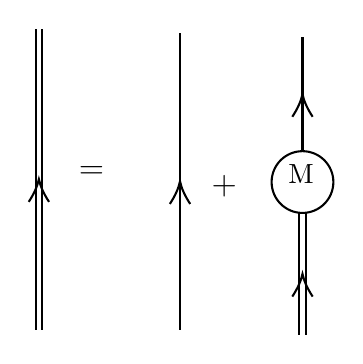
\begin{tikzpicture}[x=0.75pt,y=0.75pt,yscale=-1,xscale=1]
%uncomment if require: \path (0,300); %set diagram left start at 0, and has height of 300

%Straight Lines [id:da6679599183950475] 
\draw    (43.75,155.9) -- (43.75,10.9)(46.75,155.9) -- (46.75,10.9) ;
\draw [shift={(45.25,83.4)}, rotate = 450] [color={rgb, 255:red, 0; green, 0; blue, 0 }  ][line width=0.75]    (10.93,-4.9) .. controls (6.95,-2.3) and (3.31,-0.67) .. (0,0) .. controls (3.31,0.67) and (6.95,2.3) .. (10.93,4.9)   ;
%Straight Lines [id:da8973294663938008] 
\draw    (113.25,155.9) -- (113.25,12.9) ;
\draw [shift={(113.25,84.4)}, rotate = 450] [color={rgb, 255:red, 0; green, 0; blue, 0 }  ][line width=0.75]    (10.93,-4.9) .. controls (6.95,-2.3) and (3.31,-0.67) .. (0,0) .. controls (3.31,0.67) and (6.95,2.3) .. (10.93,4.9)   ;
%Straight Lines [id:da7528798369850997] 
\draw    (172.25,69.9) -- (172.25,14.9) ;
\draw [shift={(172.25,42.4)}, rotate = 450] [color={rgb, 255:red, 0; green, 0; blue, 0 }  ][line width=0.75]    (10.93,-4.9) .. controls (6.95,-2.3) and (3.31,-0.67) .. (0,0) .. controls (3.31,0.67) and (6.95,2.3) .. (10.93,4.9)   ;
%Shape: Circle [id:dp7507000793435626] 
\draw   (157.38,84.77) .. controls (157.38,76.56) and (164.03,69.9) .. (172.25,69.9) .. controls (180.47,69.9) and (187.13,76.56) .. (187.13,84.77) .. controls (187.13,92.99) and (180.47,99.65) .. (172.25,99.65) .. controls (164.03,99.65) and (157.38,92.99) .. (157.38,84.77) -- cycle ;
%Straight Lines [id:da663573424332869] 
\draw    (173.75,99.65) -- (173.75,158.4)(170.75,99.65) -- (170.75,158.4) ;
\draw [shift={(172.25,129.02)}, rotate = 90] [color={rgb, 255:red, 0; green, 0; blue, 0 }  ][line width=0.75]    (10.93,-4.9) .. controls (6.95,-2.3) and (3.31,-0.67) .. (0,0) .. controls (3.31,0.67) and (6.95,2.3) .. (10.93,4.9)   ;

% Text Node
\draw (63,76.02) node [anchor=north west][inner sep=0.75pt]  [font=\large]  {$=$};
% Text Node
\draw (164,75) node [anchor=north west][inner sep=0.75pt]   [align=left] {M};
% Text Node
\draw (127,80) node [anchor=north west][inner sep=0.75pt]  [font=\large] [align=left] {+};


\end{tikzpicture}

\end{center}
Finally, we substitute for $G_{0}^{+}$ and for $V_{M}$ and obtain:
\begin{equation}G^{+}(\mathbf{k}, \omega)=\frac{1}{\omega-\epsilon_{k}+i \delta-V_{M_{k k}}}=\frac{1}{\omega-\left(\epsilon_{k}+M k^{2}\right)+i \delta}\end{equation}
Comparing this with the quasi particle propagator we find
\begin{equation}\begin{array}{l}
\epsilon_{k}^{\prime}=\epsilon_{k}+M k^{2}=\left(\frac{1}{2 m}+M\right) k^{2} \\
\tau_{k}=\frac{1}{\delta}=\infty
\end{array}\end{equation}

If we consider $V_L$, we calculate the whole diagram series as 
\begin{center}
\tikzset{every picture/.style={line width=0.75pt}} %set default line width to 0.75pt        

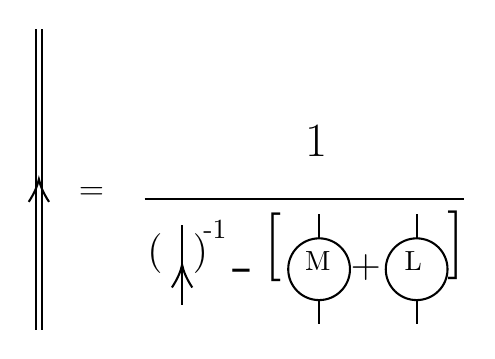
\begin{tikzpicture}[x=0.75pt,y=0.75pt,yscale=-1,xscale=1]
%uncomment if require: \path (0,300); %set diagram left start at 0, and has height of 300

%Straight Lines [id:da6679599183950475] 
\draw    (21.75,153.9) -- (21.75,8.9)(24.75,153.9) -- (24.75,8.9) ;
\draw [shift={(23.25,81.4)}, rotate = 450] [color={rgb, 255:red, 0; green, 0; blue, 0 }  ][line width=0.75]    (10.93,-4.9) .. controls (6.95,-2.3) and (3.31,-0.67) .. (0,0) .. controls (3.31,0.67) and (6.95,2.3) .. (10.93,4.9)   ;
%Shape: Circle [id:dp8530247155182938] 
\draw   (143.38,124.77) .. controls (143.38,116.56) and (150.03,109.9) .. (158.25,109.9) .. controls (166.47,109.9) and (173.13,116.56) .. (173.13,124.77) .. controls (173.13,132.99) and (166.47,139.65) .. (158.25,139.65) .. controls (150.03,139.65) and (143.38,132.99) .. (143.38,124.77) -- cycle ;
%Straight Lines [id:da5960930796514846] 
\draw    (74.25,91.02) -- (228.25,91.02) ;
%Straight Lines [id:da5321584258205649] 
\draw    (92.25,141.9) -- (92.25,103.4) ;
\draw [shift={(92.25,122.65)}, rotate = 450] [color={rgb, 255:red, 0; green, 0; blue, 0 }  ][line width=0.75]    (10.93,-4.9) .. controls (6.95,-2.3) and (3.31,-0.67) .. (0,0) .. controls (3.31,0.67) and (6.95,2.3) .. (10.93,4.9)   ;
%Straight Lines [id:da11643204321065659] 
\draw    (158.25,109.9) -- (158.25,98.4) ;
%Straight Lines [id:da8969952308596885] 
\draw    (158.25,139.65) -- (158.25,151.4) ;
%Shape: Circle [id:dp18446767982176082] 
\draw   (190.38,124.77) .. controls (190.38,116.56) and (197.03,109.9) .. (205.25,109.9) .. controls (213.47,109.9) and (220.13,116.56) .. (220.13,124.77) .. controls (220.13,132.99) and (213.47,139.65) .. (205.25,139.65) .. controls (197.03,139.65) and (190.38,132.99) .. (190.38,124.77) -- cycle ;
%Straight Lines [id:da2983905665141421] 
\draw    (205.25,109.9) -- (205.25,98.4) ;
%Straight Lines [id:da04673018570564247] 
\draw    (205.25,139.65) -- (205.25,151.4) ;

% Text Node
\draw (41,84.02) node [anchor=north west][inner sep=0.75pt]  [font=\large]  {$=$};
% Text Node
\draw (115,117) node [anchor=north west][inner sep=0.75pt]  [font=\Huge] [align=left] {\mbox{-}};
% Text Node
\draw (150,115) node [anchor=north west][inner sep=0.75pt]   [align=left] {M};
% Text Node
\draw (150,54.02) node [anchor=north west][inner sep=0.75pt]  [font=\LARGE]  {$1$};
% Text Node
\draw (96,106.02) node [anchor=north west][inner sep=0.75pt]  [font=\Large]  {$)$};
% Text Node
\draw (74,106.02) node [anchor=north west][inner sep=0.75pt]  [font=\Large]  {$($};
% Text Node
\draw (198,115) node [anchor=north west][inner sep=0.75pt]   [align=left] {L};
% Text Node
\draw (172,116) node [anchor=north west][inner sep=0.75pt]  [font=\Large] [align=left] {+};
% Text Node
\draw (130.6,96.02) node [anchor=north west][inner sep=0.75pt]  [font=\Huge] [align=left] {[};
% Text Node
\draw (218.65,95.02) node [anchor=north west][inner sep=0.75pt]  [font=\Huge] [align=left] {]};
% Text Node
\draw (101,100.02) node [anchor=north west][inner sep=0.75pt]   [align=left] {\mbox{-}1};


\end{tikzpicture}

\end{center}
or, translating:
\begin{equation}G^{+}(\mathbf{k}, \omega)=\frac{1}{\left(G_{0}^{+}\right)^{-1}-\left(V_{M_{k k}}+V_{L_{k k}}\right)}=\frac{1}{\omega-\left(\frac{k^{2}}{2 m}+M k^{2}+L k^{4}\right)+i \delta}\end{equation}

\subsection{Where the diagram expansion or the propagator really comes from}
We will now show in a rough way how the diagram expansion of $G^{+}$ in this single-particle case can be gotten from the Schrodinger equation. The first thing to realize is that \textbf{$G_{0}^{+}$ and $G^{+}$ are actually Green's functions}. Recall that if we have a differential equation of the form
\begin{equation}L \psi(\mathbf{x}, t)=f(\mathbf{x}, t)
\label{diagram-expand-exp-1}
\end{equation}
where $L$ is a linear differential operator which does not depend explicitly on $x$ or $t,$ then the Green's function, $G,$ associated with this equation is the solution of
\begin{equation}L G\left(\mathbf{x}-\mathbf{x}^{\prime}, t-t^{\prime}\right)=\delta\left(\mathbf{x}-\mathbf{x}^{\prime}\right) \delta\left(t-t^{\prime}\right)
\label{diagram-expand-exp-2}
\end{equation}
Now the unperturbed Schrodinger equation may be written
$$\left(+\frac{\nabla^{2}}{2 m}+i \frac{\partial}{\partial t}\right) \psi(\mathbf{x}, t)=0$$
Thus, the associated Green's function obeys
\begin{equation}\left(+\frac{\nabla^{2}}{2 m}+i \frac{\partial}{\partial t}\right) G\left(\mathbf{x}-\mathbf{x}^{\prime}, t-t^{\prime}\right)=\delta\left(\mathbf{x}-\mathbf{x}^{\prime}\right)\delta\left(t-t^{\prime}\right)
\label{diagram-expand-exp-3}
\end{equation}
Since
\begin{equation}G\left(x-x^{\prime}, t-t^{\prime}\right)=\int \frac{d^{3} k}{(2 \pi)^{3}} e^{i k \cdot\left(x-x^{\prime}\right)} G\left(k, t-t^{\prime}\right)
\label{diagram-expand-exp-4}
\end{equation}
and using the Fourier transform of $\delta(x-x^{\prime})$ we find that
\begin{equation}\left(-\frac{k^{2}}{2 m}+i \frac{\partial}{\partial t}\right) G\left(\mathbf{k}, t-t^{\prime}\right)=\delta\left(t-t^{\prime}\right)
\label{diagram-expand-exp-5}
\end{equation}
If we use the fact that
\begin{imp}
\begin{equation}\frac{d \theta_{x}}{d x}=\delta(x), \quad f(x) \delta(x)=f(0) \delta(x)
\label{diagram-expand-exp-6}
\end{equation}
\end{imp}
and substitute $G^+_0(\mathbf{k},\omega)=-i\theta_{t-t^{\prime}}e^{-i\epsilon_k(t=t^{\prime})}$ into (\ref{diagram-expand-exp-5}), we find the $G_0^+$ is satisfied.

In a similar way, the Shrodinger equation with a perturbing potential $V(\nabla)$
\begin{equation}\left[+\frac{\nabla^{2}}{2 m}+i \frac{\partial}{\partial t}-V(\nabla)\right] \psi(\mathbf{x}, t)=0\end{equation}
has associated Green's function as
\begin{equation}\left[-\frac{k^{2}}{2 m}+i \frac{\partial}{\partial t}-V(\mathbf{k})\right] G^{+}\left(\mathbf{k}, t-t^{\prime}\right)=\delta\left(t-t^{\prime}\right)
\label{diagram-expand-7}
\end{equation}
where $V(\mathbf{k})$ is the Fourier transform of $V(\nabla) .$ The solution to this may be written as an integral equation
\begin{equation}\boldsymbol{G}^{+}\left(\mathbf{k}, t-t^{\prime}\right)=G_{\mathbf{0}}^{+}\left(\mathbf{k}, t-t^{\prime}\right)+\int_{-\infty}^{+\infty} d t^{*} G_{0}^{+}\left(\mathbf{k}, t-t^{*}\right) V(\mathbf{k}) G^{+}\left(\mathbf{k}, t^{*}-t^{\prime}\right)
\label{diagram-expand-exp-8}
\end{equation}
This can be seen by substituting (\ref{diagram-expand-exp-8}) into (\ref{diagram-expand-7}) and use (\ref{diagram-expand-exp-5}) with $G=G^+_0$.Expanding the (\ref{diagram-expand-exp-8}) we recover the series in spacetime.

\subsection{Energy and lifetime of an electron In an Impure metal}
We will now apply the propagator method to a more realistic problem, i.e., an electron in an impure metal. For simplicity, Jet us pretend that the regularly arranged lattice ions in the metal have been removed, so that all we have left is an electron interacting with a set of N randomly distributed impurity ions, which are identical in a volume $\Omega$. If we use $\mathbf{R}_i$ to represent ion coordinates, then the potential well for an impurity at the $\mathbf{R_i}$ has the form of $W(\mathbf{r}-\mathbf{R}_i)$. Recall that $\phi(\mathbf{r})=e^{-i\mathbf{k\cdot r}}$, we have the matrix element of transitioning amplitude from $\mathbf{k}$ to $\mathbf{l}$ at $R_i$ as
\begin{equation}-i V_{\mathbf{lk}}\left(\mathbf{R}_{i}\right)=\frac{-i}{\Omega} \int d^{3} \mathbf{r} e^{-i(\mathbf{l}-\mathbf{k}) \cdot \mathbf{r}} \mathbf{W}\left(\mathbf{r}-\mathbf{R}_{i}\right)
\label{W-potential-amplitude}
\end{equation}
\redp{Now using $\mathbf{r}^{\prime}=\mathbf{r}-\mathbf{R}_i$}, we have (\ref{W-potential-amplitude}) becomes
\begin{equation}
    -iV_{\mathbf{lk}}=\frac{(-i)}{\Omega} e^{-i(\mathbf{l-k}) \cdot \mathbf{R}_{i}} \mathbf{W}_{l k}
    \label{W-potential-amplitude-2}
\end{equation}
where
$$W_{l k}=\int d^{3} \mathbf{r}^{\prime} e^{-i(\mathbf{l}-\mathbf{k}) \cdot \mathbf{r}^{\prime}} W\left(\mathbf{r}^{\prime}\right)$$
After eliminating the $i$ 's and suppressing $\omega$ 's for brevity, (noting that it is necessary to sum over all values of the intermediate momentum, $\mathbf{l}$) we have:
\begin{equation}\begin{aligned}
G^{+}\left(\mathbf{k}_{2}, \mathbf{k}_{1}\right)=& G_{0}^{+}\left(\mathbf{k}_{1}\right) \delta_{k_{1} k_{2}}+G_{0}^{+}\left(\mathbf{k}_{2}\right) \sum_{t=1}^{N} V_{k_{2} k_{1}}\left(\mathbf{R}_{i}\right) G_{0}^{+}\left(\mathbf{k}_{1}\right)+\\
&+G_{0}^{+}\left(\mathbf{k}_{2}\right)\left[\sum_{l} \sum_{i=1}^{N} V_{k_{2} l}\left(\mathbf{R}_{i}\right) G_{0}^{+}(\mathbf{l}) V_{l k_{1}}\left(\mathbf{R}_{i}\right)\right] G_{0}^{+}\left(\mathbf{k}_{1}\right)+\\
&+G_{0}^{+}\left(\mathbf{k}_{2}\right)\left[\sum_{l} \sum_{j \neq 1} V_{k_{2} l}\left(\mathbf{R}_{j}\right) G_{0}^{+}(\mathbf{l}) \sum_{i=1}^{N} V_{l k_{1}}\left(\mathbf{R}_{l}\right)\right] G_{0}^{+}\left(\mathbf{k}_{1}\right)+\cdots
\end{aligned}
\label{impurity-ion-amp-expansion}
\end{equation}
The above $G^{+}$ is for a particular set of $\mathbf{R}_{i}$ 's, and for each different set of $\mathbf{R}_{t}^{\prime}$ 's, we will get a different value of $G^{+} .$ Consider now an \bluep{ensemble consisting of all possible arrangements of impurities}. Suppose this ensemble is random, i.e., \textbf{the coordinate for the ith impurtity, $\mathbf{R}_{\mathbf{i}}$, is equally likely to be found anywhere in the volume $\Omega$.} Let us imagine that we compute $\left\langle G^{+}\right\rangle,$ the average value of $G^{+}$ for the ensemble. Clearly, for any specific arrangement, $G^{+} \neq\left\langle G^{+}\right\rangle .$ But, \redp{as is common in large systems, in the limit $N \rightarrow \infty$ (with $N / \Omega=\text { constant }),$ the ratio of the mean square fluctuation $\left(\left\langle G^{+2}\right\rangle-\left\langle G^{+}\right\rangle^{2}\right)$ to $\left\langle G^{+}\right\rangle^{2}$ will go to zero, \textbf{so that we can take $G^{+}=\left\langle G^{+}\right\rangle$ for all but a negligible number of arrangements (see Kohn and Luttinger (1957))}}. Hence our object here will be to calculate $\langle G^+\rangle$.

From \ref{impurity-ion-amp-expansion}, we have
\begin{equation}\left\langle G_{0}^{+}\left(\mathbf{k}_{2}\right) G_{0}^{+}\left(\mathbf{k}_{1}\right) \sum_{i=1}^{N} V_{k_{2} k_{1}}\left(\mathbf{R}_{i}\right)\right\rangle=G_{0}^{+}\left(\mathbf{k}_{2}\right) G_{0}^{+}\left(\mathbf{k}_{1}\right) \frac{W_{k_{2} k_{1}}}{\Omega}\left\langle\sum_{i=1}^{N} e^{-i\left(\mathbf{k}_{2}-\mathbf{k}_{1}\right) \cdot \mathbf{r}_{i}}\right\rangle
\label{impurity-1-avg}
\end{equation}
where
\begin{equation}\left\langle\sum_{t=1}^{N} e^{-i\left(\mathbf{k}_{2}-\mathbf{k}_{1}\right) \cdot \mathbf{R}_{i}}\right\rangle=\sum_{i=1}^{N} \langle e^{-i(\mathbf{k}_{2}-\mathbf{k}_{1}) \cdot \mathbf{R}_{i}}\rangle=N\langle e^{-i(\mathbf{k}_{2}-\mathbf{k}_{1}) \cdot \mathbf{R}_{i}}\rangle
\end{equation}
Since the distribution of the ions is totally random, we have
\begin{equation}
\langle e^{-i(\mathbf{k}_{2}-\mathbf{k}_{1}) \cdot \mathbf{R}_{i}}\rangle=\frac{1}{\Omega} \int d^{3} \mathbf{R}_{i} e^{-i\left(\mathbf{k}_{2}-\mathbf{k}_{1}\right) \cdot \mathbf{R}_{i}}=\frac{1}{\Omega} \times \Omega \delta_{\mathbf{k}_{2} \mathbf{k}_{1}}
\label{random-avg}
\end{equation}
\begin{mybox}
In a one-dimensional box of length $L$,
$$I \equiv \int_{-L / 2}^{+L / 2} d x \exp (-i k x)=2 k^{-1} \sin (k L / 2)$$
Because of periodic boundary conditions, the wave function at $x=0$ equals that at $x=L,$ i.e., $\exp (i k x)=\exp (i k(x+L)) .$ Hence $\exp (i k L)=1,$ or $k=2 \pi n / L$
$(n=\text { integer }) .$ Thus $I=L \delta_{k, 0} .$ Equation (\ref{random-avg}) is just the three-dimensional version of this with $\Omega=L^3$. If $\mathbf{k}$ is continuous, the integral (\ref{random-avg}) yields $(2 \pi)^{3} \delta\left(\mathbf{k}_{2}-\mathbf{k}_{1}\right),$ which is a Dirac $\delta$ -function.
\end{mybox}
Similarly, for successive scattering on the same ion, we have
\begin{equation}
    \begin{aligned}
\sum_{l} G_{0}^{+}(\mathbf{l})\left\langle\sum_{i} V_{\mathrm{k}_{2} l}\left(\mathrm{R}_{i}\right) V_{lk_{1}}\left(\mathrm{R}_{i}\right)\right\rangle &=\sum_{\mathbf{l}} G_{0}^{+}(\mathbf{l}) \frac{W_{\mathrm{k}_{2} l} W_{\mathrm{lk_1}}}{\Omega^{2}}\left\langle\sum_{\mathrm{i}} e^{-i\left(k_{2}-l+l-\mathrm{k}_{1}\right) \cdot R_{i}}\right\rangle \\
&=\frac{N}{\Omega^{2}} \sum_{l} G_{0}^{+}(\mathbf{l}) W_{\mathrm{k}_{2} l} W_{l k_{1}} \delta_{\mathrm{k}_{2} \mathrm{k}_{1}}
\end{aligned}
\label{impurity-1st-avg}
\end{equation}
It is usually more convenient to change from a sum over $\mathbf{l}$ to an integral by
\begin{imp}
\begin{equation}\sum_{l} \rightarrow \frac{\Omega}{(2 \pi)^{3}} \int d^{3} \mathbf{l}\end{equation}
The factor $\Omega /(2 \pi)^{3}$ is the density of points in $\mathrm{k}$ -space. To see this, we note that in one dimension, $k=2 \pi n / L$ $(n=\text { integer }) .$ Thus there are $L / 2 \pi$ points per unit length in $\mathbf{k}-$space in one dimension. In three dimensions we have $L^3/(2\pi)^3=\Omega/(2\pi)^3$ points per unit volume in $\mathbf{k}-$space.
\end{imp}
\ref{impurity-1st-avg} now becomes
$$=\frac{N}{\Omega} \int \frac{d^{3} \mathbf{l}}{(2 \pi)^{3}} G_{0}^{+}(1) W_{k_{2}l} W_{l k_{1}} \delta_{k_{2} k_{1}}$$
The two successive scattering term from different ions contains the average 
$$\begin{array}{l}
\sum_{l} G_{0}^{+}(l)\left\langle\sum_{l, j\neq i} V_{k_{2} l}\left(R_{i}\right) V_{lk_1}{\left(R_{i}\right)}\right\rangle \\
\quad=\sum_{l} G_{0}^{+}(l) \frac{W_{k_{2} l} W_{l k_{1}}}{\Omega^{2}}\left\langle\sum_{l, j \neq i} e^{-i\left(k_{2}-\mathbf{l}\right) \cdot R_{j}} e^{-i\left(\mathbf{l}-k_{1}\right) \cdot R_{i}}\right)\\
\quad=\sum_{l} G_{0}^{+}(1) \frac{W_{k_{2} l} W_{l k_{1}}}{\Omega^{2}} N(N-1)\int \frac{d^{3} \mathbf{R}_{j}}{\Omega} \int \frac{d^{3} \mathbf{R}_{i}}{\Omega}e^{-i\left(k_{2}-\mathbf{l}\right) \cdot R_{j}} e^{-i(\mathbf{l}-k_{1}) \cdot R_{i}})\\
\quad\approx\left(\frac{N}{\Omega}\right)^{2} \sum_{l} G_{0}^{+}(l) W_{k_{2} l} W_{l k_{1}} \delta_{k_{2} l} \delta_{l k_{2}}\\
\quad=\left(\frac{N}{\Omega}\right)^{2} G_{0}^{+}\left(\mathbf{k}_{1}\right) W_{k_{1} k_{1}}^{2} \delta_{k_{2} k_{1}}
\end{array}$$
With the aid of these results, we can write out the series for the averaged propagator. It helps here to introduce a couple of new diagram conventions. First of all, we use just an empty circle to represent $V_{lk}(\mathbf{R}_i)$, for the transition probability amplitude $W_{lk}$ Secondly, \bluep{\textbf{because each group of two or more successive scatterings at the same ion has an associated density factor $N/\Omega$,}} we connect successive circles representing the same ion by dotted
lines. (Note that a single scattering also has this factor associated with it.) Thus, taking the $\delta$-functions into account, and letting $\mathbf{k}_1=\mathbf{k}=\mathbf{k}_2$, we have for the averaged propagator:

\begin{equation}
    \tikzset{every picture/.style={line width=0.75pt}} %set default line width to 0.75pt        
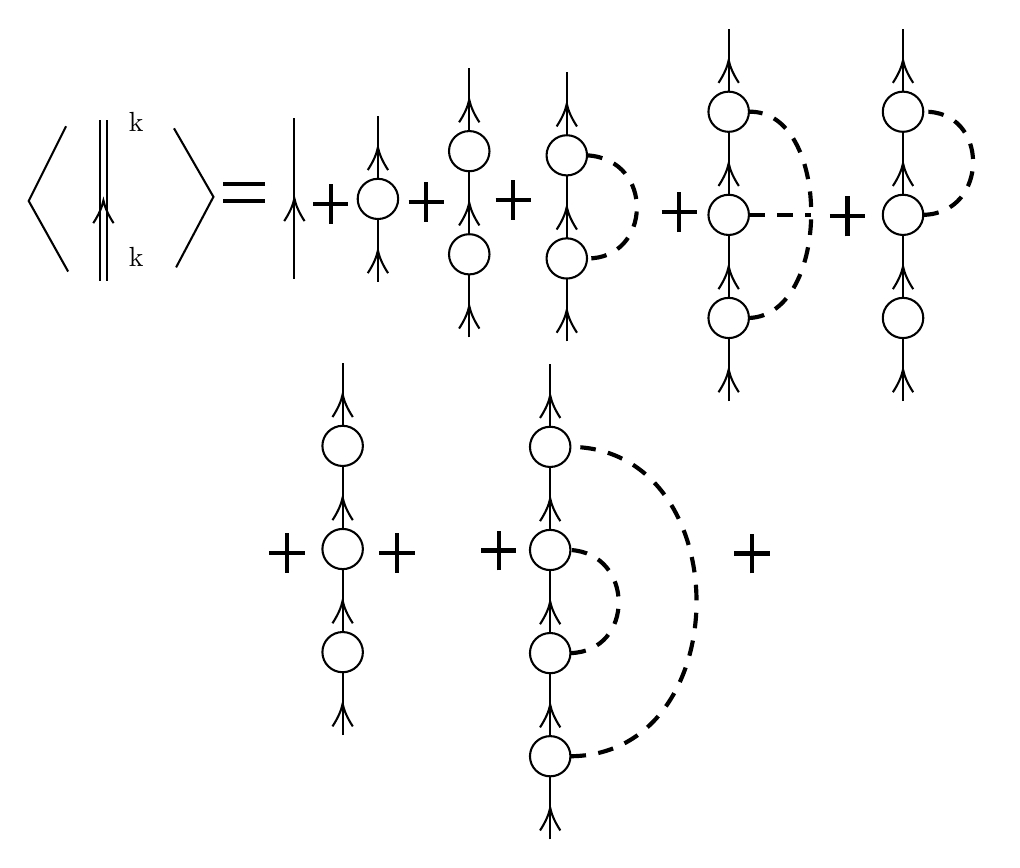
\begin{tikzpicture}[x=0.75pt,y=0.75pt,yscale=-1,xscale=1]
%uncomment if require: \path (0,410); %set diagram left start at 0, and has height of 410

%Straight Lines [id:da6679599183950475] 
\draw    (42.75,129.9) -- (42.75,52.4)(45.75,129.9) -- (45.75,52.4) ;
\draw [shift={(44.25,91.15)}, rotate = 450] [color={rgb, 255:red, 0; green, 0; blue, 0 }  ][line width=0.75]    (10.93,-4.9) .. controls (6.95,-2.3) and (3.31,-0.67) .. (0,0) .. controls (3.31,0.67) and (6.95,2.3) .. (10.93,4.9)   ;
%Straight Lines [id:da96866989164835] 
\draw    (78.25,56.4) -- (97.25,89.4) -- (79.25,123.4) ;
%Straight Lines [id:da6934326937577064] 
\draw    (26.25,55.4) -- (8.25,91.4) -- (27.25,125.4) ;
%Straight Lines [id:da3013274600825496] 
\draw [line width=1.5]    (102,83.02) -- (122.25,83.02) ;
%Straight Lines [id:da002431265709683772] 
\draw [line width=1.5]    (102,91.4) -- (122.25,91.4) ;

%Straight Lines [id:da5008643601850559] 
\draw    (136.25,128.9) -- (136.25,51.4) ;
\draw [shift={(136.25,90.15)}, rotate = 450] [color={rgb, 255:red, 0; green, 0; blue, 0 }  ][line width=0.75]    (10.93,-4.9) .. controls (6.95,-2.3) and (3.31,-0.67) .. (0,0) .. controls (3.31,0.67) and (6.95,2.3) .. (10.93,4.9)   ;
%Straight Lines [id:da6945756947603086] 
\draw    (176.5,80.72) -- (176.5,50.4) ;
\draw [shift={(176.5,65.56)}, rotate = 450] [color={rgb, 255:red, 0; green, 0; blue, 0 }  ][line width=0.75]    (10.93,-4.9) .. controls (6.95,-2.3) and (3.31,-0.67) .. (0,0) .. controls (3.31,0.67) and (6.95,2.3) .. (10.93,4.9)   ;
%Shape: Ellipse [id:dp3530646460829052] 
\draw   (166.75,90.4) .. controls (166.75,85.05) and (171.12,80.72) .. (176.5,80.72) .. controls (181.88,80.72) and (186.25,85.05) .. (186.25,90.4) .. controls (186.25,95.75) and (181.88,100.08) .. (176.5,100.08) .. controls (171.12,100.08) and (166.75,95.75) .. (166.75,90.4) -- cycle ;
%Straight Lines [id:da43208207245118435] 
\draw    (176.5,130.4) -- (176.5,100.08) ;
\draw [shift={(176.5,115.24)}, rotate = 450] [color={rgb, 255:red, 0; green, 0; blue, 0 }  ][line width=0.75]    (10.93,-4.9) .. controls (6.95,-2.3) and (3.31,-0.67) .. (0,0) .. controls (3.31,0.67) and (6.95,2.3) .. (10.93,4.9)   ;

%Straight Lines [id:da7828111751257385] 
\draw    (220.5,57.72) -- (220.5,27.4) ;
\draw [shift={(220.5,42.56)}, rotate = 450] [color={rgb, 255:red, 0; green, 0; blue, 0 }  ][line width=0.75]    (10.93,-4.9) .. controls (6.95,-2.3) and (3.31,-0.67) .. (0,0) .. controls (3.31,0.67) and (6.95,2.3) .. (10.93,4.9)   ;
%Shape: Ellipse [id:dp6295020134353576] 
\draw   (210.75,67.4) .. controls (210.75,62.05) and (215.12,57.72) .. (220.5,57.72) .. controls (225.88,57.72) and (230.25,62.05) .. (230.25,67.4) .. controls (230.25,72.75) and (225.88,77.08) .. (220.5,77.08) .. controls (215.12,77.08) and (210.75,72.75) .. (210.75,67.4) -- cycle ;
%Straight Lines [id:da5190411567838193] 
\draw    (220.5,107.4) -- (220.5,77.08) ;
\draw [shift={(220.5,92.24)}, rotate = 450] [color={rgb, 255:red, 0; green, 0; blue, 0 }  ][line width=0.75]    (10.93,-4.9) .. controls (6.95,-2.3) and (3.31,-0.67) .. (0,0) .. controls (3.31,0.67) and (6.95,2.3) .. (10.93,4.9)   ;

%Shape: Ellipse [id:dp1856254885258023] 
\draw   (210.75,117.08) .. controls (210.75,111.74) and (215.12,107.4) .. (220.5,107.4) .. controls (225.88,107.4) and (230.25,111.74) .. (230.25,117.08) .. controls (230.25,122.43) and (225.88,126.77) .. (220.5,126.77) .. controls (215.12,126.77) and (210.75,122.43) .. (210.75,117.08) -- cycle ;
%Straight Lines [id:da12064415501164083] 
\draw    (220.5,157.08) -- (220.5,126.77) ;
\draw [shift={(220.5,141.93)}, rotate = 450] [color={rgb, 255:red, 0; green, 0; blue, 0 }  ][line width=0.75]    (10.93,-4.9) .. controls (6.95,-2.3) and (3.31,-0.67) .. (0,0) .. controls (3.31,0.67) and (6.95,2.3) .. (10.93,4.9)   ;
%Straight Lines [id:da7079596940921928] 
\draw    (267.5,59.72) -- (267.5,29.4) ;
\draw [shift={(267.5,44.56)}, rotate = 450] [color={rgb, 255:red, 0; green, 0; blue, 0 }  ][line width=0.75]    (10.93,-4.9) .. controls (6.95,-2.3) and (3.31,-0.67) .. (0,0) .. controls (3.31,0.67) and (6.95,2.3) .. (10.93,4.9)   ;
%Shape: Ellipse [id:dp22478419986022313] 
\draw   (257.75,69.4) .. controls (257.75,64.05) and (262.12,59.72) .. (267.5,59.72) .. controls (272.88,59.72) and (277.25,64.05) .. (277.25,69.4) .. controls (277.25,74.75) and (272.88,79.08) .. (267.5,79.08) .. controls (262.12,79.08) and (257.75,74.75) .. (257.75,69.4) -- cycle ;
%Straight Lines [id:da11608178895592369] 
\draw    (267.5,109.4) -- (267.5,79.08) ;
\draw [shift={(267.5,94.24)}, rotate = 450] [color={rgb, 255:red, 0; green, 0; blue, 0 }  ][line width=0.75]    (10.93,-4.9) .. controls (6.95,-2.3) and (3.31,-0.67) .. (0,0) .. controls (3.31,0.67) and (6.95,2.3) .. (10.93,4.9)   ;

%Shape: Ellipse [id:dp33421438233375045] 
\draw   (257.75,119.08) .. controls (257.75,113.74) and (262.12,109.4) .. (267.5,109.4) .. controls (272.88,109.4) and (277.25,113.74) .. (277.25,119.08) .. controls (277.25,124.43) and (272.88,128.77) .. (267.5,128.77) .. controls (262.12,128.77) and (257.75,124.43) .. (257.75,119.08) -- cycle ;
%Straight Lines [id:da8470461387935158] 
\draw    (267.5,159.08) -- (267.5,128.77) ;
\draw [shift={(267.5,143.93)}, rotate = 450] [color={rgb, 255:red, 0; green, 0; blue, 0 }  ][line width=0.75]    (10.93,-4.9) .. controls (6.95,-2.3) and (3.31,-0.67) .. (0,0) .. controls (3.31,0.67) and (6.95,2.3) .. (10.93,4.9)   ;
%Straight Lines [id:da5580045724596926] 
\draw [line width=1.5]    (145.25,92.8) -- (162.25,92.8) ;
%Straight Lines [id:da21350536390327923] 
\draw [line width=1.5]    (153.75,102.4) -- (153.75,83.21) ;

%Straight Lines [id:da8624253903000908] 
\draw [line width=1.5]    (191.25,91.8) -- (208.25,91.8) ;
%Straight Lines [id:da39200924475692256] 
\draw [line width=1.5]    (199.75,101.4) -- (199.75,82.21) ;

%Straight Lines [id:da11442905940915027] 
\draw [line width=1.5]    (233.25,90.8) -- (250.25,90.8) ;
%Straight Lines [id:da6458220565812314] 
\draw [line width=1.5]    (241.75,100.4) -- (241.75,81.21) ;

%Curve Lines [id:da5905027576335966] 
\draw [line width=1.5]  [dash pattern={on 5.63pt off 4.5pt}]  (277.25,69.4) .. controls (310.25,71.4) and (308.25,119.4) .. (277.25,119.08) ;
%Straight Lines [id:da9968425195966377] 
\draw    (345.5,38.72) -- (345.5,8.4) ;
\draw [shift={(345.5,23.56)}, rotate = 450] [color={rgb, 255:red, 0; green, 0; blue, 0 }  ][line width=0.75]    (10.93,-4.9) .. controls (6.95,-2.3) and (3.31,-0.67) .. (0,0) .. controls (3.31,0.67) and (6.95,2.3) .. (10.93,4.9)   ;
%Shape: Ellipse [id:dp9509322965168189] 
\draw   (335.75,48.4) .. controls (335.75,43.05) and (340.12,38.72) .. (345.5,38.72) .. controls (350.88,38.72) and (355.25,43.05) .. (355.25,48.4) .. controls (355.25,53.75) and (350.88,58.08) .. (345.5,58.08) .. controls (340.12,58.08) and (335.75,53.75) .. (335.75,48.4) -- cycle ;
%Straight Lines [id:da08673873782145747] 
\draw    (345.5,88.4) -- (345.5,58.08) ;
\draw [shift={(345.5,73.24)}, rotate = 450] [color={rgb, 255:red, 0; green, 0; blue, 0 }  ][line width=0.75]    (10.93,-4.9) .. controls (6.95,-2.3) and (3.31,-0.67) .. (0,0) .. controls (3.31,0.67) and (6.95,2.3) .. (10.93,4.9)   ;

%Shape: Ellipse [id:dp8921785518031183] 
\draw   (335.75,98.08) .. controls (335.75,92.74) and (340.12,88.4) .. (345.5,88.4) .. controls (350.88,88.4) and (355.25,92.74) .. (355.25,98.08) .. controls (355.25,103.43) and (350.88,107.77) .. (345.5,107.77) .. controls (340.12,107.77) and (335.75,103.43) .. (335.75,98.08) -- cycle ;
%Straight Lines [id:da5781140789642911] 
\draw    (345.5,138.08) -- (345.5,107.77) ;
\draw [shift={(345.5,122.93)}, rotate = 450] [color={rgb, 255:red, 0; green, 0; blue, 0 }  ][line width=0.75]    (10.93,-4.9) .. controls (6.95,-2.3) and (3.31,-0.67) .. (0,0) .. controls (3.31,0.67) and (6.95,2.3) .. (10.93,4.9)   ;
%Shape: Ellipse [id:dp9670986903241016] 
\draw   (335.75,147.77) .. controls (335.75,142.42) and (340.12,138.08) .. (345.5,138.08) .. controls (350.88,138.08) and (355.25,142.42) .. (355.25,147.77) .. controls (355.25,153.12) and (350.88,157.45) .. (345.5,157.45) .. controls (340.12,157.45) and (335.75,153.12) .. (335.75,147.77) -- cycle ;
%Straight Lines [id:da9751245477461478] 
\draw    (345.5,187.77) -- (345.5,157.45) ;
\draw [shift={(345.5,172.61)}, rotate = 450] [color={rgb, 255:red, 0; green, 0; blue, 0 }  ][line width=0.75]    (10.93,-4.9) .. controls (6.95,-2.3) and (3.31,-0.67) .. (0,0) .. controls (3.31,0.67) and (6.95,2.3) .. (10.93,4.9)   ;
%Curve Lines [id:da845705807763435] 
\draw [line width=1.5]  [dash pattern={on 5.63pt off 4.5pt}]  (355.25,147.77) .. controls (395.25,146.4) and (395.25,47.4) .. (355.25,48.4) ;
%Straight Lines [id:da3256851388470269] 
\draw [line width=1.5]  [dash pattern={on 5.63pt off 4.5pt}]  (355.25,98.08) -- (385.25,98.08) ;
%Straight Lines [id:da09806150660985813] 
\draw [line width=1.5]    (313.25,96.8) -- (330.25,96.8) ;
%Straight Lines [id:da8319212817021413] 
\draw [line width=1.5]    (321.75,106.4) -- (321.75,87.21) ;

%Straight Lines [id:da17267749447821656] 
\draw    (429.5,38.72) -- (429.5,8.4) ;
\draw [shift={(429.5,23.56)}, rotate = 450] [color={rgb, 255:red, 0; green, 0; blue, 0 }  ][line width=0.75]    (10.93,-4.9) .. controls (6.95,-2.3) and (3.31,-0.67) .. (0,0) .. controls (3.31,0.67) and (6.95,2.3) .. (10.93,4.9)   ;
%Shape: Ellipse [id:dp6338000815403856] 
\draw   (419.75,48.4) .. controls (419.75,43.05) and (424.12,38.72) .. (429.5,38.72) .. controls (434.88,38.72) and (439.25,43.05) .. (439.25,48.4) .. controls (439.25,53.75) and (434.88,58.08) .. (429.5,58.08) .. controls (424.12,58.08) and (419.75,53.75) .. (419.75,48.4) -- cycle ;
%Straight Lines [id:da6359368270166951] 
\draw    (429.5,88.4) -- (429.5,58.08) ;
\draw [shift={(429.5,73.24)}, rotate = 450] [color={rgb, 255:red, 0; green, 0; blue, 0 }  ][line width=0.75]    (10.93,-4.9) .. controls (6.95,-2.3) and (3.31,-0.67) .. (0,0) .. controls (3.31,0.67) and (6.95,2.3) .. (10.93,4.9)   ;

%Shape: Ellipse [id:dp8160936873445316] 
\draw   (419.75,98.08) .. controls (419.75,92.74) and (424.12,88.4) .. (429.5,88.4) .. controls (434.88,88.4) and (439.25,92.74) .. (439.25,98.08) .. controls (439.25,103.43) and (434.88,107.77) .. (429.5,107.77) .. controls (424.12,107.77) and (419.75,103.43) .. (419.75,98.08) -- cycle ;
%Straight Lines [id:da9286035597952149] 
\draw    (429.5,138.08) -- (429.5,107.77) ;
\draw [shift={(429.5,122.93)}, rotate = 450] [color={rgb, 255:red, 0; green, 0; blue, 0 }  ][line width=0.75]    (10.93,-4.9) .. controls (6.95,-2.3) and (3.31,-0.67) .. (0,0) .. controls (3.31,0.67) and (6.95,2.3) .. (10.93,4.9)   ;
%Shape: Ellipse [id:dp07506037090452533] 
\draw   (419.75,147.77) .. controls (419.75,142.42) and (424.12,138.08) .. (429.5,138.08) .. controls (434.88,138.08) and (439.25,142.42) .. (439.25,147.77) .. controls (439.25,153.12) and (434.88,157.45) .. (429.5,157.45) .. controls (424.12,157.45) and (419.75,153.12) .. (419.75,147.77) -- cycle ;
%Straight Lines [id:da3948811378599879] 
\draw    (429.5,187.77) -- (429.5,157.45) ;
\draw [shift={(429.5,172.61)}, rotate = 450] [color={rgb, 255:red, 0; green, 0; blue, 0 }  ][line width=0.75]    (10.93,-4.9) .. controls (6.95,-2.3) and (3.31,-0.67) .. (0,0) .. controls (3.31,0.67) and (6.95,2.3) .. (10.93,4.9)   ;
%Curve Lines [id:da8457780212222412] 
\draw [line width=1.5]  [dash pattern={on 5.63pt off 4.5pt}]  (439.25,98.08) .. controls (471.25,97.4) and (471.25,47.4) .. (439.25,48.4) ;
%Straight Lines [id:da7096138963389558] 
\draw [line width=1.5]    (394.25,98.8) -- (411.25,98.8) ;
%Straight Lines [id:da5958532372098427] 
\draw [line width=1.5]    (402.75,108.4) -- (402.75,89.21) ;

%Straight Lines [id:da2873192509320337] 
\draw    (159.5,199.72) -- (159.5,169.4) ;
\draw [shift={(159.5,184.56)}, rotate = 450] [color={rgb, 255:red, 0; green, 0; blue, 0 }  ][line width=0.75]    (10.93,-4.9) .. controls (6.95,-2.3) and (3.31,-0.67) .. (0,0) .. controls (3.31,0.67) and (6.95,2.3) .. (10.93,4.9)   ;
%Shape: Ellipse [id:dp427210573936433] 
\draw   (149.75,209.4) .. controls (149.75,204.05) and (154.12,199.72) .. (159.5,199.72) .. controls (164.88,199.72) and (169.25,204.05) .. (169.25,209.4) .. controls (169.25,214.75) and (164.88,219.08) .. (159.5,219.08) .. controls (154.12,219.08) and (149.75,214.75) .. (149.75,209.4) -- cycle ;
%Straight Lines [id:da46462676043390816] 
\draw    (159.5,249.4) -- (159.5,219.08) ;
\draw [shift={(159.5,234.24)}, rotate = 450] [color={rgb, 255:red, 0; green, 0; blue, 0 }  ][line width=0.75]    (10.93,-4.9) .. controls (6.95,-2.3) and (3.31,-0.67) .. (0,0) .. controls (3.31,0.67) and (6.95,2.3) .. (10.93,4.9)   ;

%Shape: Ellipse [id:dp8330119640828625] 
\draw   (149.75,259.08) .. controls (149.75,253.74) and (154.12,249.4) .. (159.5,249.4) .. controls (164.88,249.4) and (169.25,253.74) .. (169.25,259.08) .. controls (169.25,264.43) and (164.88,268.77) .. (159.5,268.77) .. controls (154.12,268.77) and (149.75,264.43) .. (149.75,259.08) -- cycle ;
%Straight Lines [id:da6375532829975131] 
\draw    (159.5,299.08) -- (159.5,268.77) ;
\draw [shift={(159.5,283.93)}, rotate = 450] [color={rgb, 255:red, 0; green, 0; blue, 0 }  ][line width=0.75]    (10.93,-4.9) .. controls (6.95,-2.3) and (3.31,-0.67) .. (0,0) .. controls (3.31,0.67) and (6.95,2.3) .. (10.93,4.9)   ;
%Shape: Ellipse [id:dp5126298651489208] 
\draw   (149.75,308.77) .. controls (149.75,303.42) and (154.12,299.08) .. (159.5,299.08) .. controls (164.88,299.08) and (169.25,303.42) .. (169.25,308.77) .. controls (169.25,314.12) and (164.88,318.45) .. (159.5,318.45) .. controls (154.12,318.45) and (149.75,314.12) .. (149.75,308.77) -- cycle ;
%Straight Lines [id:da3195137766405717] 
\draw    (159.5,348.77) -- (159.5,318.45) ;
\draw [shift={(159.5,333.61)}, rotate = 450] [color={rgb, 255:red, 0; green, 0; blue, 0 }  ][line width=0.75]    (10.93,-4.9) .. controls (6.95,-2.3) and (3.31,-0.67) .. (0,0) .. controls (3.31,0.67) and (6.95,2.3) .. (10.93,4.9)   ;
%Straight Lines [id:da24487221646253365] 
\draw [line width=1.5]    (124.25,260.8) -- (141.25,260.8) ;
%Straight Lines [id:da5139191095297375] 
\draw [line width=1.5]    (132.75,270.4) -- (132.75,251.21) ;

%Straight Lines [id:da5879011823878417] 
\draw [line width=1.5]    (177.25,260.8) -- (194.25,260.8) ;
%Straight Lines [id:da7804073333032313] 
\draw [line width=1.5]    (185.75,270.4) -- (185.75,251.21) ;

%Straight Lines [id:da0562657792203165] 
\draw [line width=1.5]    (226.25,259.8) -- (243.25,259.8) ;
%Straight Lines [id:da35139000015559874] 
\draw [line width=1.5]    (234.75,269.4) -- (234.75,250.21) ;

%Straight Lines [id:da29474857872821825] 
\draw    (259.5,200.18) -- (259.5,169.86) ;
\draw [shift={(259.5,185.02)}, rotate = 450] [color={rgb, 255:red, 0; green, 0; blue, 0 }  ][line width=0.75]    (10.93,-4.9) .. controls (6.95,-2.3) and (3.31,-0.67) .. (0,0) .. controls (3.31,0.67) and (6.95,2.3) .. (10.93,4.9)   ;
%Shape: Ellipse [id:dp26134073591403817] 
\draw   (249.75,209.86) .. controls (249.75,204.52) and (254.12,200.18) .. (259.5,200.18) .. controls (264.88,200.18) and (269.25,204.52) .. (269.25,209.86) .. controls (269.25,215.21) and (264.88,219.55) .. (259.5,219.55) .. controls (254.12,219.55) and (249.75,215.21) .. (249.75,209.86) -- cycle ;
%Straight Lines [id:da16694755775136938] 
\draw    (259.5,249.86) -- (259.5,219.55) ;
\draw [shift={(259.5,234.71)}, rotate = 450] [color={rgb, 255:red, 0; green, 0; blue, 0 }  ][line width=0.75]    (10.93,-4.9) .. controls (6.95,-2.3) and (3.31,-0.67) .. (0,0) .. controls (3.31,0.67) and (6.95,2.3) .. (10.93,4.9)   ;

%Shape: Ellipse [id:dp10810512476445211] 
\draw   (249.75,259.55) .. controls (249.75,254.2) and (254.12,249.86) .. (259.5,249.86) .. controls (264.88,249.86) and (269.25,254.2) .. (269.25,259.55) .. controls (269.25,264.9) and (264.88,269.23) .. (259.5,269.23) .. controls (254.12,269.23) and (249.75,264.9) .. (249.75,259.55) -- cycle ;
%Straight Lines [id:da3762019551905843] 
\draw    (259.5,299.55) -- (259.5,269.23) ;
\draw [shift={(259.5,284.39)}, rotate = 450] [color={rgb, 255:red, 0; green, 0; blue, 0 }  ][line width=0.75]    (10.93,-4.9) .. controls (6.95,-2.3) and (3.31,-0.67) .. (0,0) .. controls (3.31,0.67) and (6.95,2.3) .. (10.93,4.9)   ;
%Shape: Ellipse [id:dp7544795909371296] 
\draw   (249.75,309.23) .. controls (249.75,303.88) and (254.12,299.55) .. (259.5,299.55) .. controls (264.88,299.55) and (269.25,303.88) .. (269.25,309.23) .. controls (269.25,314.58) and (264.88,318.92) .. (259.5,318.92) .. controls (254.12,318.92) and (249.75,314.58) .. (249.75,309.23) -- cycle ;
%Straight Lines [id:da13163878925416705] 
\draw    (259.5,349.23) -- (259.5,318.92) ;
\draw [shift={(259.5,334.08)}, rotate = 450] [color={rgb, 255:red, 0; green, 0; blue, 0 }  ][line width=0.75]    (10.93,-4.9) .. controls (6.95,-2.3) and (3.31,-0.67) .. (0,0) .. controls (3.31,0.67) and (6.95,2.3) .. (10.93,4.9)   ;
%Straight Lines [id:da4226970698781941] 
\draw [line width=1.5]    (348.25,261.27) -- (365.25,261.27) ;
%Straight Lines [id:da4222013167527927] 
\draw [line width=1.5]    (356.75,270.86) -- (356.75,251.67) ;

%Shape: Ellipse [id:dp6254769479483138] 
\draw   (249.75,358.92) .. controls (249.75,353.57) and (254.12,349.23) .. (259.5,349.23) .. controls (264.88,349.23) and (269.25,353.57) .. (269.25,358.92) .. controls (269.25,364.27) and (264.88,368.6) .. (259.5,368.6) .. controls (254.12,368.6) and (249.75,364.27) .. (249.75,358.92) -- cycle ;
%Straight Lines [id:da19493897948698158] 
\draw    (259.5,398.92) -- (259.5,368.6) ;
\draw [shift={(259.5,383.76)}, rotate = 450] [color={rgb, 255:red, 0; green, 0; blue, 0 }  ][line width=0.75]    (10.93,-4.9) .. controls (6.95,-2.3) and (3.31,-0.67) .. (0,0) .. controls (3.31,0.67) and (6.95,2.3) .. (10.93,4.9)   ;
%Curve Lines [id:da08525623172658137] 
\draw [line width=1.5]  [dash pattern={on 5.63pt off 4.5pt}]  (269.25,358.92) .. controls (350.25,358.4) and (350.25,210.4) .. (269.25,209.86) ;
%Curve Lines [id:da05679915324880036] 
\draw [line width=1.5]  [dash pattern={on 5.63pt off 4.5pt}]  (269.25,309.23) .. controls (300.25,308.4) and (300.25,261.4) .. (269.25,259.55) ;

% Text Node
\draw (55,47.02) node [anchor=north west][inner sep=0.75pt]   [align=left] {k};
% Text Node
\draw (55,112.02) node [anchor=north west][inner sep=0.75pt]   [align=left] {k};
% Text Node
\draw (462,76.02) node [anchor=north west][inner sep=0.75pt]    {$\dotsc $};
% Text Node
\draw (195,236.02) node [anchor=north west][inner sep=0.75pt]    {$\dotsc $};
% Text Node
\draw (364,242.02) node [anchor=north west][inner sep=0.75pt]    {$\dotsc $};


\end{tikzpicture}
\label{whole-impurity-diagram-series}
\end{equation}

This may be translated with the dictionary in Table  Note that in this table, \bluep{there is no factor $\Omega^{-1}$ in front of $\int d^{3} 1 /(2 \pi)^{3}$ because all $\Omega^{-1}$ factors are already included in the $(N / \Omega)$ factor in line 4 of the table.}

\begin{table}[H]
\caption{Dictionary for electron propagating through a system of randomly distributed impurity ions}
\label{tab:impurity-dict}
\centering
\begin{tabular}{|c|c|}
\hline
Diagram Element          & Factor                                                                               \\ \hline



\tikzset{every picture/.style={line width=0.75pt}} %set default line width to 0.75pt        

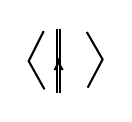
\begin{tikzpicture}[x=0.75pt,y=0.75pt,yscale=-1,xscale=1,scale=0.4, transform shape]
%uncomment if require: \path (0,410); %set diagram left start at 0, and has height of 410

%Straight Lines [id:da6679599183950475] 
\draw    (42.75,129.9) -- (42.75,52.4)(45.75,129.9) -- (45.75,52.4) ;
\draw [shift={(44.25,91.15)}, rotate = 450] [color={rgb, 255:red, 0; green, 0; blue, 0 }  ][line width=0.75]    (10.93,-4.9) .. controls (6.95,-2.3) and (3.31,-0.67) .. (0,0) .. controls (3.31,0.67) and (6.95,2.3) .. (10.93,4.9)   ;
%Straight Lines [id:da96866989164835] 
\draw    (78.25,56.4) -- (97.25,89.4) -- (79.25,123.4) ;
%Straight Lines [id:da6934326937577064] 
\draw    (26.25,55.4) -- (8.25,91.4) -- (27.25,125.4) ;
\end{tikzpicture}
                        & $i\langle G^+(\mathbf{k},\omega)\rangle$                                             \\ \hline



\tikzset{every picture/.style={line width=0.75pt}} %set default line width to 0.75pt        

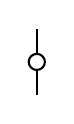
\begin{tikzpicture}[x=0.75pt,y=0.75pt,yscale=-1,xscale=1,scale=0.4, transform shape]
%uncomment if require: \path (0,410); %set diagram left start at 0, and has height of 410

%Straight Lines [id:da28668922103226246] 
\draw    (505.5,288.72) -- (505.5,258.4) ;
%Shape: Ellipse [id:dp08452238525628197] 
\draw   (495.75,298.4) .. controls (495.75,293.05) and (500.12,288.72) .. (505.5,288.72) .. controls (510.88,288.72) and (515.25,293.05) .. (515.25,298.4) .. controls (515.25,303.75) and (510.88,308.08) .. (505.5,308.08) .. controls (500.12,308.08) and (495.75,303.75) .. (495.75,298.4) -- cycle ;
%Straight Lines [id:da3057641306656801] 
\draw    (505.5,338.4) -- (505.5,308.08) ;




\end{tikzpicture}
                        & $-iW_{lk}$                                                                           \\ \hline



\tikzset{every picture/.style={line width=0.75pt}} %set default line width to 0.75pt        

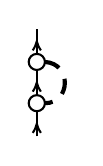
\begin{tikzpicture}[x=0.75pt,y=0.75pt,yscale=-1,xscale=1,scale=0.4, transform shape]
%uncomment if require: \path (0,410); %set diagram left start at 0, and has height of 410

%Straight Lines [id:da7079596940921928] 
\draw    (267.5,59.72) -- (267.5,29.4) ;
\draw [shift={(267.5,44.56)}, rotate = 450] [color={rgb, 255:red, 0; green, 0; blue, 0 }  ][line width=0.75]    (10.93,-4.9) .. controls (6.95,-2.3) and (3.31,-0.67) .. (0,0) .. controls (3.31,0.67) and (6.95,2.3) .. (10.93,4.9)   ;
%Shape: Ellipse [id:dp22478419986022313] 
\draw   (257.75,69.4) .. controls (257.75,64.05) and (262.12,59.72) .. (267.5,59.72) .. controls (272.88,59.72) and (277.25,64.05) .. (277.25,69.4) .. controls (277.25,74.75) and (272.88,79.08) .. (267.5,79.08) .. controls (262.12,79.08) and (257.75,74.75) .. (257.75,69.4) -- cycle ;
%Straight Lines [id:da11608178895592369] 
\draw    (267.5,109.4) -- (267.5,79.08) ;
\draw [shift={(267.5,94.24)}, rotate = 450] [color={rgb, 255:red, 0; green, 0; blue, 0 }  ][line width=0.75]    (10.93,-4.9) .. controls (6.95,-2.3) and (3.31,-0.67) .. (0,0) .. controls (3.31,0.67) and (6.95,2.3) .. (10.93,4.9)   ;

%Shape: Ellipse [id:dp33421438233375045] 
\draw   (257.75,119.08) .. controls (257.75,113.74) and (262.12,109.4) .. (267.5,109.4) .. controls (272.88,109.4) and (277.25,113.74) .. (277.25,119.08) .. controls (277.25,124.43) and (272.88,128.77) .. (267.5,128.77) .. controls (262.12,128.77) and (257.75,124.43) .. (257.75,119.08) -- cycle ;
%Straight Lines [id:da8470461387935158] 
\draw    (267.5,159.08) -- (267.5,128.77) ;
\draw [shift={(267.5,143.93)}, rotate = 450] [color={rgb, 255:red, 0; green, 0; blue, 0 }  ][line width=0.75]    (10.93,-4.9) .. controls (6.95,-2.3) and (3.31,-0.67) .. (0,0) .. controls (3.31,0.67) and (6.95,2.3) .. (10.93,4.9)   ;
%Curve Lines [id:da5905027576335966] 
\draw [line width=1.5]  [dash pattern={on 5.63pt off 4.5pt}]  (277.25,69.4) .. controls (310.25,71.4) and (308.25,119.4) .. (277.25,119.08) ;




\end{tikzpicture}
                        & factor $N/\Omega$                                                                    \\ \hline
intermediate momentum, I & $\int \frac{d^{3} l}{(2 \pi)^{3}}$                                                   \\ \hline


    \tikzset{every picture/.style={line width=0.75pt}} %set default line width to 0.75pt        

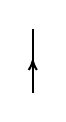
\begin{tikzpicture}[x=0.75pt,y=0.75pt,yscale=-1,xscale=1,scale=0.4, transform shape]
%uncomment if require: \path (0,410); %set diagram left start at 0, and has height of 410

%Straight Lines [id:da5008643601850559] 
\draw    (136.25,128.9) -- (136.25,51.4) ;
\draw [shift={(136.25,90.15)}, rotate = 450] [color={rgb, 255:red, 0; green, 0; blue, 0 }  ][line width=0.75]    (10.93,-4.9) .. controls (6.95,-2.3) and (3.31,-0.67) .. (0,0) .. controls (3.31,0.67) and (6.95,2.3) .. (10.93,4.9)   ;
\end{tikzpicture}
                       & $i G_{0}^{+}(\mathbf{k}, \omega)=\frac{i}{\omega-\varepsilon_{\mathrm{k}}+i \delta}$ \\ \hline
\end{tabular}
\end{table}

Let's evaluate \ref{whole-impurity-diagram-series} by assuming the most important processes are single scattering, and double scattering by the same impurity. This means that diagrams containing more than two successive scatterings off the same ion are neglected.The partial sum may easily be carried out and yields
\begin{equation}
\tikzset{every picture/.style={line width=0.75pt}} %set default line width to 0.75pt        
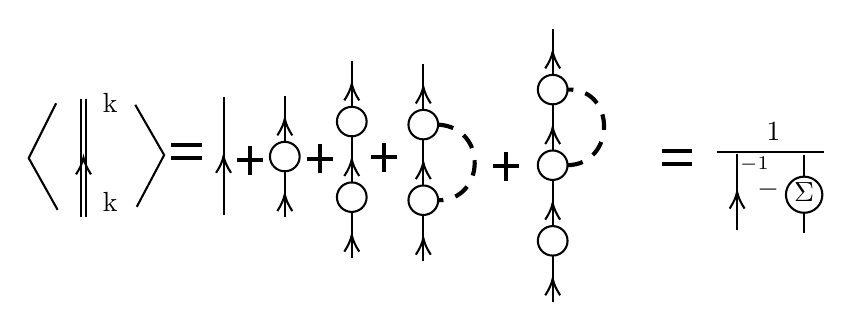
\begin{tikzpicture}[x=0.55pt,y=0.55pt,yscale=-1,xscale=1]
%uncomment if require: \path (0,410); %set diagram left start at 0, and has height of 410

%Straight Lines [id:da6679599183950475] 
\draw    (42.75,129.9) -- (42.75,52.4)(45.75,129.9) -- (45.75,52.4) ;
\draw [shift={(44.25,91.15)}, rotate = 450] [color={rgb, 255:red, 0; green, 0; blue, 0 }  ][line width=0.75]    (10.93,-4.9) .. controls (6.95,-2.3) and (3.31,-0.67) .. (0,0) .. controls (3.31,0.67) and (6.95,2.3) .. (10.93,4.9)   ;
%Straight Lines [id:da96866989164835] 
\draw    (78.25,56.4) -- (97.25,89.4) -- (79.25,123.4) ;
%Straight Lines [id:da6934326937577064] 
\draw    (26.25,55.4) -- (8.25,91.4) -- (27.25,125.4) ;
%Straight Lines [id:da3013274600825496] 
\draw [line width=1.5]    (102,83.02) -- (122.25,83.02) ;
%Straight Lines [id:da002431265709683772] 
\draw [line width=1.5]    (102,91.4) -- (122.25,91.4) ;

%Straight Lines [id:da5008643601850559] 
\draw    (136.25,128.9) -- (136.25,51.4) ;
\draw [shift={(136.25,90.15)}, rotate = 450] [color={rgb, 255:red, 0; green, 0; blue, 0 }  ][line width=0.75]    (10.93,-4.9) .. controls (6.95,-2.3) and (3.31,-0.67) .. (0,0) .. controls (3.31,0.67) and (6.95,2.3) .. (10.93,4.9)   ;
%Straight Lines [id:da6945756947603086] 
\draw    (176.5,80.72) -- (176.5,50.4) ;
\draw [shift={(176.5,65.56)}, rotate = 450] [color={rgb, 255:red, 0; green, 0; blue, 0 }  ][line width=0.75]    (10.93,-4.9) .. controls (6.95,-2.3) and (3.31,-0.67) .. (0,0) .. controls (3.31,0.67) and (6.95,2.3) .. (10.93,4.9)   ;
%Shape: Ellipse [id:dp3530646460829052] 
\draw   (166.75,90.4) .. controls (166.75,85.05) and (171.12,80.72) .. (176.5,80.72) .. controls (181.88,80.72) and (186.25,85.05) .. (186.25,90.4) .. controls (186.25,95.75) and (181.88,100.08) .. (176.5,100.08) .. controls (171.12,100.08) and (166.75,95.75) .. (166.75,90.4) -- cycle ;
%Straight Lines [id:da43208207245118435] 
\draw    (176.5,130.4) -- (176.5,100.08) ;
\draw [shift={(176.5,115.24)}, rotate = 450] [color={rgb, 255:red, 0; green, 0; blue, 0 }  ][line width=0.75]    (10.93,-4.9) .. controls (6.95,-2.3) and (3.31,-0.67) .. (0,0) .. controls (3.31,0.67) and (6.95,2.3) .. (10.93,4.9)   ;

%Straight Lines [id:da7828111751257385] 
\draw    (220.5,57.72) -- (220.5,27.4) ;
\draw [shift={(220.5,42.56)}, rotate = 450] [color={rgb, 255:red, 0; green, 0; blue, 0 }  ][line width=0.75]    (10.93,-4.9) .. controls (6.95,-2.3) and (3.31,-0.67) .. (0,0) .. controls (3.31,0.67) and (6.95,2.3) .. (10.93,4.9)   ;
%Shape: Ellipse [id:dp6295020134353576] 
\draw   (210.75,67.4) .. controls (210.75,62.05) and (215.12,57.72) .. (220.5,57.72) .. controls (225.88,57.72) and (230.25,62.05) .. (230.25,67.4) .. controls (230.25,72.75) and (225.88,77.08) .. (220.5,77.08) .. controls (215.12,77.08) and (210.75,72.75) .. (210.75,67.4) -- cycle ;
%Straight Lines [id:da5190411567838193] 
\draw    (220.5,107.4) -- (220.5,77.08) ;
\draw [shift={(220.5,92.24)}, rotate = 450] [color={rgb, 255:red, 0; green, 0; blue, 0 }  ][line width=0.75]    (10.93,-4.9) .. controls (6.95,-2.3) and (3.31,-0.67) .. (0,0) .. controls (3.31,0.67) and (6.95,2.3) .. (10.93,4.9)   ;

%Shape: Ellipse [id:dp1856254885258023] 
\draw   (210.75,117.08) .. controls (210.75,111.74) and (215.12,107.4) .. (220.5,107.4) .. controls (225.88,107.4) and (230.25,111.74) .. (230.25,117.08) .. controls (230.25,122.43) and (225.88,126.77) .. (220.5,126.77) .. controls (215.12,126.77) and (210.75,122.43) .. (210.75,117.08) -- cycle ;
%Straight Lines [id:da12064415501164083] 
\draw    (220.5,157.08) -- (220.5,126.77) ;
\draw [shift={(220.5,141.93)}, rotate = 450] [color={rgb, 255:red, 0; green, 0; blue, 0 }  ][line width=0.75]    (10.93,-4.9) .. controls (6.95,-2.3) and (3.31,-0.67) .. (0,0) .. controls (3.31,0.67) and (6.95,2.3) .. (10.93,4.9)   ;
%Straight Lines [id:da7079596940921928] 
\draw    (267.5,59.72) -- (267.5,29.4) ;
\draw [shift={(267.5,44.56)}, rotate = 450] [color={rgb, 255:red, 0; green, 0; blue, 0 }  ][line width=0.75]    (10.93,-4.9) .. controls (6.95,-2.3) and (3.31,-0.67) .. (0,0) .. controls (3.31,0.67) and (6.95,2.3) .. (10.93,4.9)   ;
%Shape: Ellipse [id:dp22478419986022313] 
\draw   (257.75,69.4) .. controls (257.75,64.05) and (262.12,59.72) .. (267.5,59.72) .. controls (272.88,59.72) and (277.25,64.05) .. (277.25,69.4) .. controls (277.25,74.75) and (272.88,79.08) .. (267.5,79.08) .. controls (262.12,79.08) and (257.75,74.75) .. (257.75,69.4) -- cycle ;
%Straight Lines [id:da11608178895592369] 
\draw    (267.5,109.4) -- (267.5,79.08) ;
\draw [shift={(267.5,94.24)}, rotate = 450] [color={rgb, 255:red, 0; green, 0; blue, 0 }  ][line width=0.75]    (10.93,-4.9) .. controls (6.95,-2.3) and (3.31,-0.67) .. (0,0) .. controls (3.31,0.67) and (6.95,2.3) .. (10.93,4.9)   ;

%Shape: Ellipse [id:dp33421438233375045] 
\draw   (257.75,119.08) .. controls (257.75,113.74) and (262.12,109.4) .. (267.5,109.4) .. controls (272.88,109.4) and (277.25,113.74) .. (277.25,119.08) .. controls (277.25,124.43) and (272.88,128.77) .. (267.5,128.77) .. controls (262.12,128.77) and (257.75,124.43) .. (257.75,119.08) -- cycle ;
%Straight Lines [id:da8470461387935158] 
\draw    (267.5,159.08) -- (267.5,128.77) ;
\draw [shift={(267.5,143.93)}, rotate = 450] [color={rgb, 255:red, 0; green, 0; blue, 0 }  ][line width=0.75]    (10.93,-4.9) .. controls (6.95,-2.3) and (3.31,-0.67) .. (0,0) .. controls (3.31,0.67) and (6.95,2.3) .. (10.93,4.9)   ;
%Straight Lines [id:da5580045724596926] 
\draw [line width=1.5]    (145.25,92.8) -- (162.25,92.8) ;
%Straight Lines [id:da21350536390327923] 
\draw [line width=1.5]    (153.75,102.4) -- (153.75,83.21) ;

%Straight Lines [id:da8624253903000908] 
\draw [line width=1.5]    (191.25,91.8) -- (208.25,91.8) ;
%Straight Lines [id:da39200924475692256] 
\draw [line width=1.5]    (199.75,101.4) -- (199.75,82.21) ;

%Straight Lines [id:da11442905940915027] 
\draw [line width=1.5]    (233.25,90.8) -- (250.25,90.8) ;
%Straight Lines [id:da6458220565812314] 
\draw [line width=1.5]    (241.75,100.4) -- (241.75,81.21) ;

%Curve Lines [id:da5905027576335966] 
\draw [line width=1.5]  [dash pattern={on 5.63pt off 4.5pt}]  (277.25,69.4) .. controls (310.25,71.4) and (308.25,119.4) .. (277.25,119.08) ;
%Straight Lines [id:da09806150660985813] 
\draw [line width=1.5]    (313.25,96.8) -- (330.25,96.8) ;
%Straight Lines [id:da8319212817021413] 
\draw [line width=1.5]    (321.75,106.4) -- (321.75,87.21) ;

%Straight Lines [id:da17267749447821656] 
\draw    (352.5,36.72) -- (352.5,6.4) ;
\draw [shift={(352.5,21.56)}, rotate = 450] [color={rgb, 255:red, 0; green, 0; blue, 0 }  ][line width=0.75]    (10.93,-4.9) .. controls (6.95,-2.3) and (3.31,-0.67) .. (0,0) .. controls (3.31,0.67) and (6.95,2.3) .. (10.93,4.9)   ;
%Shape: Ellipse [id:dp6338000815403856] 
\draw   (342.75,46.4) .. controls (342.75,41.05) and (347.12,36.72) .. (352.5,36.72) .. controls (357.88,36.72) and (362.25,41.05) .. (362.25,46.4) .. controls (362.25,51.75) and (357.88,56.08) .. (352.5,56.08) .. controls (347.12,56.08) and (342.75,51.75) .. (342.75,46.4) -- cycle ;
%Straight Lines [id:da6359368270166951] 
\draw    (352.5,86.4) -- (352.5,56.08) ;
\draw [shift={(352.5,71.24)}, rotate = 450] [color={rgb, 255:red, 0; green, 0; blue, 0 }  ][line width=0.75]    (10.93,-4.9) .. controls (6.95,-2.3) and (3.31,-0.67) .. (0,0) .. controls (3.31,0.67) and (6.95,2.3) .. (10.93,4.9)   ;

%Shape: Ellipse [id:dp8160936873445316] 
\draw   (342.75,96.08) .. controls (342.75,90.74) and (347.12,86.4) .. (352.5,86.4) .. controls (357.88,86.4) and (362.25,90.74) .. (362.25,96.08) .. controls (362.25,101.43) and (357.88,105.77) .. (352.5,105.77) .. controls (347.12,105.77) and (342.75,101.43) .. (342.75,96.08) -- cycle ;
%Straight Lines [id:da9286035597952149] 
\draw    (352.5,136.08) -- (352.5,105.77) ;
\draw [shift={(352.5,120.93)}, rotate = 450] [color={rgb, 255:red, 0; green, 0; blue, 0 }  ][line width=0.75]    (10.93,-4.9) .. controls (6.95,-2.3) and (3.31,-0.67) .. (0,0) .. controls (3.31,0.67) and (6.95,2.3) .. (10.93,4.9)   ;
%Shape: Ellipse [id:dp07506037090452533] 
\draw   (342.75,145.77) .. controls (342.75,140.42) and (347.12,136.08) .. (352.5,136.08) .. controls (357.88,136.08) and (362.25,140.42) .. (362.25,145.77) .. controls (362.25,151.12) and (357.88,155.45) .. (352.5,155.45) .. controls (347.12,155.45) and (342.75,151.12) .. (342.75,145.77) -- cycle ;
%Straight Lines [id:da3948811378599879] 
\draw    (352.5,185.77) -- (352.5,155.45) ;
\draw [shift={(352.5,170.61)}, rotate = 450] [color={rgb, 255:red, 0; green, 0; blue, 0 }  ][line width=0.75]    (10.93,-4.9) .. controls (6.95,-2.3) and (3.31,-0.67) .. (0,0) .. controls (3.31,0.67) and (6.95,2.3) .. (10.93,4.9)   ;
%Curve Lines [id:da8457780212222412] 
\draw [line width=1.5]  [dash pattern={on 5.63pt off 4.5pt}]  (362.25,96.08) .. controls (394.25,95.4) and (394.25,45.4) .. (362.25,46.4) ;
%Straight Lines [id:da17632381462435154] 
\draw [line width=1.5]    (424,87.02) -- (444.25,87.02) ;
%Straight Lines [id:da2860027932323479] 
\draw [line width=1.5]    (424,95.4) -- (444.25,95.4) ;

%Straight Lines [id:da3219886118472701] 
\draw    (473.67,138.63) -- (473.67,88.63) ;
\draw [shift={(473.67,113.63)}, rotate = 450] [color={rgb, 255:red, 0; green, 0; blue, 0 }  ][line width=0.75]    (10.93,-4.9) .. controls (6.95,-2.3) and (3.31,-0.67) .. (0,0) .. controls (3.31,0.67) and (6.95,2.3) .. (10.93,4.9)   ;
%Straight Lines [id:da7155527870457447] 
\draw    (517.71,103.59) -- (517.71,89.63) ;
%Shape: Ellipse [id:dp6470069643074525] 
\draw   (505.75,115.47) .. controls (505.75,108.91) and (511.1,103.59) .. (517.71,103.59) .. controls (524.31,103.59) and (529.67,108.91) .. (529.67,115.47) .. controls (529.67,122.03) and (524.31,127.35) .. (517.71,127.35) .. controls (511.1,127.35) and (505.75,122.03) .. (505.75,115.47) -- cycle ;
%Straight Lines [id:da765234496553557] 
\draw    (517.71,140.63) -- (517.71,127.35) ;
%Straight Lines [id:da9234724283302328] 
\draw    (460.67,87.63) -- (530.67,87.63) ;


% Text Node
\draw (55,47.02) node [anchor=north west][inner sep=0.75pt]   [align=left] {k};
% Text Node
\draw (55,112.02) node [anchor=north west][inner sep=0.75pt]   [align=left] {k};
% Text Node
\draw (385,85.02) node [anchor=north west][inner sep=0.75pt]    {$\dotsc $};
% Text Node
\draw (491,66.3) node [anchor=north west][inner sep=0.75pt]    {$1$};
% Text Node
\draw (485,104.3) node [anchor=north west][inner sep=0.75pt]    {$-$};
% Text Node
\draw (473.67,88.63) node [anchor=north west][inner sep=0.75pt]    {$^{-1}$};
% Text Node
\draw (509,105.3) node [anchor=north west][inner sep=0.75pt]    {$\Sigma $};
\end{tikzpicture}
\label{single-impurity-series}
\end{equation}
where 
\begin{center}
\tikzset{every picture/.style={line width=0.75pt}} %set default line width to 0.75pt        
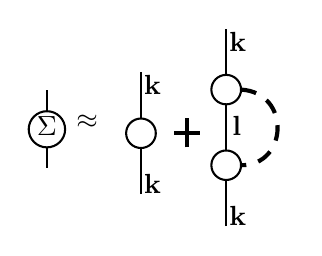
\begin{tikzpicture}[x=0.55pt,y=0.55pt,yscale=-1,xscale=1]
%uncomment if require: \path (0,410); %set diagram left start at 0, and has height of 410

%Straight Lines [id:da2478555353047407] 
\draw    (57.71,237.59) -- (57.71,223.63) ;
%Shape: Ellipse [id:dp8195879996221702] 
\draw   (45.75,249.47) .. controls (45.75,242.91) and (51.1,237.59) .. (57.71,237.59) .. controls (64.31,237.59) and (69.67,242.91) .. (69.67,249.47) .. controls (69.67,256.03) and (64.31,261.35) .. (57.71,261.35) .. controls (51.1,261.35) and (45.75,256.03) .. (45.75,249.47) -- cycle ;
%Straight Lines [id:da49340395084618693] 
\draw    (57.71,274.63) -- (57.71,261.35) ;
%Straight Lines [id:da7965677357458768] 
\draw    (119.5,242.4) -- (119.5,212.08) ;
%Shape: Ellipse [id:dp5834867502072995] 
\draw   (109.75,252.08) .. controls (109.75,246.74) and (114.12,242.4) .. (119.5,242.4) .. controls (124.88,242.4) and (129.25,246.74) .. (129.25,252.08) .. controls (129.25,257.43) and (124.88,261.77) .. (119.5,261.77) .. controls (114.12,261.77) and (109.75,257.43) .. (109.75,252.08) -- cycle ;
%Straight Lines [id:da26210627528994135] 
\draw    (119.5,292.08) -- (119.5,261.77) ;
%Straight Lines [id:da5450531939398274] 
\draw    (175.5,213.72) -- (175.5,183.4) ;
%Shape: Ellipse [id:dp7406102462871901] 
\draw   (165.75,223.4) .. controls (165.75,218.05) and (170.12,213.72) .. (175.5,213.72) .. controls (180.88,213.72) and (185.25,218.05) .. (185.25,223.4) .. controls (185.25,228.75) and (180.88,233.08) .. (175.5,233.08) .. controls (170.12,233.08) and (165.75,228.75) .. (165.75,223.4) -- cycle ;
%Straight Lines [id:da10558237608158416] 
\draw    (175.5,263.4) -- (175.5,233.08) ;
%Shape: Ellipse [id:dp052195730584338906] 
\draw   (165.75,273.08) .. controls (165.75,267.74) and (170.12,263.4) .. (175.5,263.4) .. controls (180.88,263.4) and (185.25,267.74) .. (185.25,273.08) .. controls (185.25,278.43) and (180.88,282.77) .. (175.5,282.77) .. controls (170.12,282.77) and (165.75,278.43) .. (165.75,273.08) -- cycle ;
%Straight Lines [id:da620708222735995] 
\draw    (175.5,313.08) -- (175.5,282.77) ;
%Straight Lines [id:da3887554298477651] 
\draw [line width=1.5]    (141.25,251.8) -- (158.25,251.8) ;
%Straight Lines [id:da3055944791539196] 
\draw [line width=1.5]    (149.75,261.4) -- (149.75,242.21) ;

%Curve Lines [id:da439299640958546] 
\draw [line width=1.5]  [dash pattern={on 5.63pt off 4.5pt}]  (185.25,223.4) .. controls (218.25,225.4) and (216.25,273.4) .. (185.25,273.08) ;

% Text Node
\draw (49,239.3) node [anchor=north west][inner sep=0.75pt]    {$\Sigma $};
% Text Node
\draw (119.5,212.08) node [anchor=north west][inner sep=0.75pt]   [align=left] {\textbf{k}};
% Text Node
\draw (75,238.3) node [anchor=north west][inner sep=0.75pt]    {$\approx $};
% Text Node
\draw (119.5,276.93) node [anchor=north west][inner sep=0.75pt]   [align=left] {\textbf{k}};
% Text Node
\draw (175.5,183.4) node [anchor=north west][inner sep=0.75pt]   [align=left] {\textbf{k}};
% Text Node
\draw (175.5,297.93) node [anchor=north west][inner sep=0.75pt]   [align=left] {\textbf{k}};
% Text Node
\draw (177.5,239.08) node [anchor=north west][inner sep=0.75pt]   [align=left] {\textbf{l}};
\end{tikzpicture}
\end{center}
Note that the complete series for \Circled{$\Sigma$} is
\begin{center}
\tikzset{every picture/.style={line width=0.75pt}} %set default line width to 0.75pt        
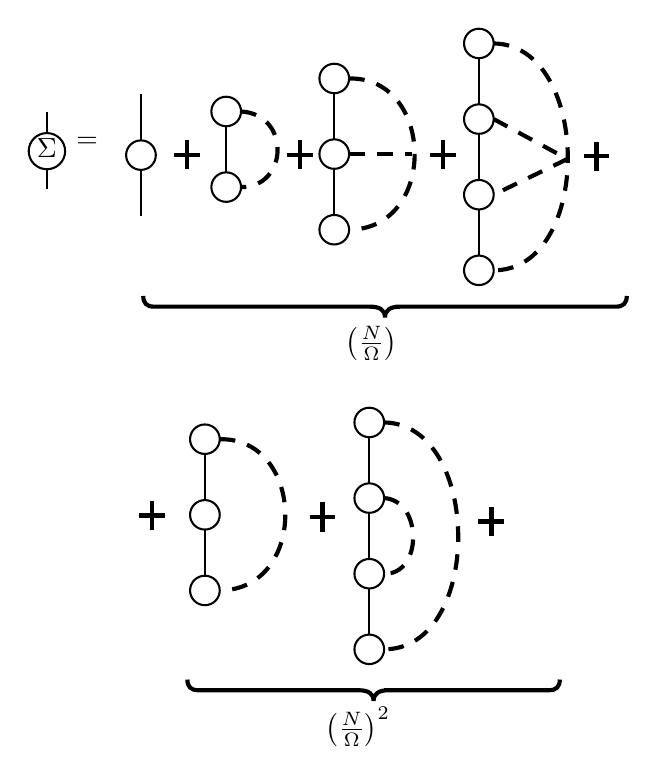
\begin{tikzpicture}[x=0.55pt,y=0.55pt,yscale=-1,xscale=1]
%uncomment if require: \path (0,705); %set diagram left start at 0, and has height of 705

%Straight Lines [id:da2478555353047407] 
\draw    (47.71,269.59) -- (47.71,255.63) ;
%Shape: Ellipse [id:dp8195879996221702] 
\draw   (35.75,281.47) .. controls (35.75,274.91) and (41.1,269.59) .. (47.71,269.59) .. controls (54.31,269.59) and (59.67,274.91) .. (59.67,281.47) .. controls (59.67,288.03) and (54.31,293.35) .. (47.71,293.35) .. controls (41.1,293.35) and (35.75,288.03) .. (35.75,281.47) -- cycle ;
%Straight Lines [id:da49340395084618693] 
\draw    (47.71,306.63) -- (47.71,293.35) ;
%Straight Lines [id:da7965677357458768] 
\draw    (109.5,274.4) -- (109.5,244.08) ;
%Shape: Ellipse [id:dp5834867502072995] 
\draw   (99.75,284.08) .. controls (99.75,278.74) and (104.12,274.4) .. (109.5,274.4) .. controls (114.88,274.4) and (119.25,278.74) .. (119.25,284.08) .. controls (119.25,289.43) and (114.88,293.77) .. (109.5,293.77) .. controls (104.12,293.77) and (99.75,289.43) .. (99.75,284.08) -- cycle ;
%Straight Lines [id:da26210627528994135] 
\draw    (109.5,324.08) -- (109.5,293.77) ;
%Shape: Ellipse [id:dp7406102462871901] 
\draw   (155.75,255.4) .. controls (155.75,250.05) and (160.12,245.72) .. (165.5,245.72) .. controls (170.88,245.72) and (175.25,250.05) .. (175.25,255.4) .. controls (175.25,260.75) and (170.88,265.08) .. (165.5,265.08) .. controls (160.12,265.08) and (155.75,260.75) .. (155.75,255.4) -- cycle ;
%Straight Lines [id:da10558237608158416] 
\draw    (165.5,295.4) -- (165.5,265.08) ;
%Shape: Ellipse [id:dp052195730584338906] 
\draw   (155.75,305.08) .. controls (155.75,299.74) and (160.12,295.4) .. (165.5,295.4) .. controls (170.88,295.4) and (175.25,299.74) .. (175.25,305.08) .. controls (175.25,310.43) and (170.88,314.77) .. (165.5,314.77) .. controls (160.12,314.77) and (155.75,310.43) .. (155.75,305.08) -- cycle ;
%Straight Lines [id:da3887554298477651] 
\draw [line width=1.5]    (131.25,283.8) -- (148.25,283.8) ;
%Straight Lines [id:da3055944791539196] 
\draw [line width=1.5]    (139.75,293.4) -- (139.75,274.21) ;

%Curve Lines [id:da439299640958546] 
\draw [line width=1.5]  [dash pattern={on 5.63pt off 4.5pt}]  (175.25,255.4) .. controls (208.25,257.4) and (206.25,305.4) .. (175.25,305.08) ;
%Shape: Ellipse [id:dp7383206567205944] 
\draw   (226.75,283.4) .. controls (226.75,278.05) and (231.12,273.72) .. (236.5,273.72) .. controls (241.88,273.72) and (246.25,278.05) .. (246.25,283.4) .. controls (246.25,288.75) and (241.88,293.08) .. (236.5,293.08) .. controls (231.12,293.08) and (226.75,288.75) .. (226.75,283.4) -- cycle ;
%Straight Lines [id:da38047468848179744] 
\draw    (236.5,323.4) -- (236.5,293.08) ;
%Shape: Ellipse [id:dp3403133897193449] 
\draw   (226.75,333.08) .. controls (226.75,327.74) and (231.12,323.4) .. (236.5,323.4) .. controls (241.88,323.4) and (246.25,327.74) .. (246.25,333.08) .. controls (246.25,338.43) and (241.88,342.77) .. (236.5,342.77) .. controls (231.12,342.77) and (226.75,338.43) .. (226.75,333.08) -- cycle ;
%Curve Lines [id:da007009060601548378] 
\draw [line width=1.5]  [dash pattern={on 5.63pt off 4.5pt}]  (246.25,233.72) .. controls (302.67,232.63) and (304.67,332.63) .. (246.25,333.08) ;
%Shape: Ellipse [id:dp35771829373861763] 
\draw   (226.75,233.72) .. controls (226.75,228.37) and (231.12,224.03) .. (236.5,224.03) .. controls (241.88,224.03) and (246.25,228.37) .. (246.25,233.72) .. controls (246.25,239.06) and (241.88,243.4) .. (236.5,243.4) .. controls (231.12,243.4) and (226.75,239.06) .. (226.75,233.72) -- cycle ;
%Straight Lines [id:da9875841078417118] 
\draw    (236.5,273.72) -- (236.5,243.4) ;
%Straight Lines [id:da7015118023288028] 
\draw [line width=1.5]  [dash pattern={on 5.63pt off 4.5pt}]  (246.25,283.4) -- (287.67,283.4) ;
%Straight Lines [id:da4960628325151931] 
\draw [line width=1.5]    (205.25,283.8) -- (222.25,283.8) ;
%Straight Lines [id:da6480371797669408] 
\draw [line width=1.5]    (213.75,293.4) -- (213.75,274.21) ;

%Shape: Ellipse [id:dp7003520544377538] 
\draw   (321.75,260.4) .. controls (321.75,255.05) and (326.12,250.72) .. (331.5,250.72) .. controls (336.88,250.72) and (341.25,255.05) .. (341.25,260.4) .. controls (341.25,265.75) and (336.88,270.08) .. (331.5,270.08) .. controls (326.12,270.08) and (321.75,265.75) .. (321.75,260.4) -- cycle ;
%Straight Lines [id:da30398624837511] 
\draw    (331.5,300.4) -- (331.5,270.08) ;
%Shape: Ellipse [id:dp0013092697739560677] 
\draw   (321.75,310.08) .. controls (321.75,304.74) and (326.12,300.4) .. (331.5,300.4) .. controls (336.88,300.4) and (341.25,304.74) .. (341.25,310.08) .. controls (341.25,315.43) and (336.88,319.77) .. (331.5,319.77) .. controls (326.12,319.77) and (321.75,315.43) .. (321.75,310.08) -- cycle ;
%Curve Lines [id:da1762989116442294] 
\draw [line width=1.5]  [dash pattern={on 5.63pt off 4.5pt}]  (341.25,210.72) .. controls (405.67,211.63) and (406.67,359.63) .. (341.25,359.77) ;
%Shape: Ellipse [id:dp0919059432356526] 
\draw   (321.75,210.72) .. controls (321.75,205.37) and (326.12,201.03) .. (331.5,201.03) .. controls (336.88,201.03) and (341.25,205.37) .. (341.25,210.72) .. controls (341.25,216.06) and (336.88,220.4) .. (331.5,220.4) .. controls (326.12,220.4) and (321.75,216.06) .. (321.75,210.72) -- cycle ;
%Straight Lines [id:da4592700821469805] 
\draw    (331.5,250.72) -- (331.5,220.4) ;
%Straight Lines [id:da4092399922684642] 
\draw [line width=1.5]  [dash pattern={on 5.63pt off 4.5pt}]  (341.25,260.4) -- (389.67,286.63) ;
%Shape: Ellipse [id:dp8221836318702264] 
\draw   (321.75,359.77) .. controls (321.75,354.42) and (326.12,350.08) .. (331.5,350.08) .. controls (336.88,350.08) and (341.25,354.42) .. (341.25,359.77) .. controls (341.25,365.12) and (336.88,369.45) .. (331.5,369.45) .. controls (326.12,369.45) and (321.75,365.12) .. (321.75,359.77) -- cycle ;
%Straight Lines [id:da7228735126740514] 
\draw    (331.5,350.08) -- (331.5,319.77) ;
%Straight Lines [id:da5303593504365808] 
\draw [line width=1.5]  [dash pattern={on 5.63pt off 4.5pt}]  (389.67,286.63) -- (341.25,310.08) ;
%Straight Lines [id:da5698850434080588] 
\draw [line width=1.5]    (299.25,283.8) -- (316.25,283.8) ;
%Straight Lines [id:da4432963135610114] 
\draw [line width=1.5]    (307.75,293.4) -- (307.75,274.21) ;

%Straight Lines [id:da2415266398742839] 
\draw [line width=1.5]    (400.25,284.8) -- (417.25,284.8) ;
%Straight Lines [id:da4340372921474619] 
\draw [line width=1.5]    (408.75,294.4) -- (408.75,275.21) ;

%Shape: Brace [id:dp6448676796499818] 
\draw  [line width=1.5]  (111,376.63) .. controls (111,381.3) and (113.33,383.63) .. (118,383.63) -- (259.83,383.63) .. controls (266.5,383.63) and (269.83,385.96) .. (269.83,390.63) .. controls (269.83,385.96) and (273.16,383.63) .. (279.83,383.63)(276.83,383.63) -- (421.67,383.63) .. controls (426.34,383.63) and (428.67,381.3) .. (428.67,376.63) ;
%Straight Lines [id:da07410677749346861] 
\draw [line width=1.5]    (108.25,520.8) -- (125.25,520.8) ;
%Straight Lines [id:da700700060848846] 
\draw [line width=1.5]    (116.75,530.4) -- (116.75,511.21) ;

%Shape: Ellipse [id:dp25309314883514067] 
\draw   (141.75,520.4) .. controls (141.75,515.05) and (146.12,510.72) .. (151.5,510.72) .. controls (156.88,510.72) and (161.25,515.05) .. (161.25,520.4) .. controls (161.25,525.75) and (156.88,530.08) .. (151.5,530.08) .. controls (146.12,530.08) and (141.75,525.75) .. (141.75,520.4) -- cycle ;
%Straight Lines [id:da15361398879570853] 
\draw    (151.5,560.4) -- (151.5,530.08) ;
%Shape: Ellipse [id:dp11922541802264952] 
\draw   (141.75,570.08) .. controls (141.75,564.74) and (146.12,560.4) .. (151.5,560.4) .. controls (156.88,560.4) and (161.25,564.74) .. (161.25,570.08) .. controls (161.25,575.43) and (156.88,579.77) .. (151.5,579.77) .. controls (146.12,579.77) and (141.75,575.43) .. (141.75,570.08) -- cycle ;
%Curve Lines [id:da6846534275233958] 
\draw [line width=1.5]  [dash pattern={on 5.63pt off 4.5pt}]  (161.25,470.72) .. controls (217.67,469.63) and (219.67,569.63) .. (161.25,570.08) ;
%Shape: Ellipse [id:dp8919508088411173] 
\draw   (141.75,470.72) .. controls (141.75,465.37) and (146.12,461.03) .. (151.5,461.03) .. controls (156.88,461.03) and (161.25,465.37) .. (161.25,470.72) .. controls (161.25,476.06) and (156.88,480.4) .. (151.5,480.4) .. controls (146.12,480.4) and (141.75,476.06) .. (141.75,470.72) -- cycle ;
%Straight Lines [id:da9808659240915968] 
\draw    (151.5,510.72) -- (151.5,480.4) ;
%Shape: Ellipse [id:dp6898707679738483] 
\draw   (249.75,509.4) .. controls (249.75,504.05) and (254.12,499.72) .. (259.5,499.72) .. controls (264.88,499.72) and (269.25,504.05) .. (269.25,509.4) .. controls (269.25,514.75) and (264.88,519.08) .. (259.5,519.08) .. controls (254.12,519.08) and (249.75,514.75) .. (249.75,509.4) -- cycle ;
%Straight Lines [id:da3999992844031298] 
\draw    (259.5,549.4) -- (259.5,519.08) ;
%Shape: Ellipse [id:dp4709695539942117] 
\draw   (249.75,559.08) .. controls (249.75,553.74) and (254.12,549.4) .. (259.5,549.4) .. controls (264.88,549.4) and (269.25,553.74) .. (269.25,559.08) .. controls (269.25,564.43) and (264.88,568.77) .. (259.5,568.77) .. controls (254.12,568.77) and (249.75,564.43) .. (249.75,559.08) -- cycle ;
%Curve Lines [id:da940049566421093] 
\draw [line width=1.5]  [dash pattern={on 5.63pt off 4.5pt}]  (269.25,459.72) .. controls (333.67,460.63) and (334.67,608.63) .. (269.25,608.77) ;
%Shape: Ellipse [id:dp6253341496158781] 
\draw   (249.75,459.72) .. controls (249.75,454.37) and (254.12,450.03) .. (259.5,450.03) .. controls (264.88,450.03) and (269.25,454.37) .. (269.25,459.72) .. controls (269.25,465.06) and (264.88,469.4) .. (259.5,469.4) .. controls (254.12,469.4) and (249.75,465.06) .. (249.75,459.72) -- cycle ;
%Straight Lines [id:da8751810296393059] 
\draw    (259.5,499.72) -- (259.5,469.4) ;
%Shape: Ellipse [id:dp8407456531271822] 
\draw   (249.75,608.77) .. controls (249.75,603.42) and (254.12,599.08) .. (259.5,599.08) .. controls (264.88,599.08) and (269.25,603.42) .. (269.25,608.77) .. controls (269.25,614.12) and (264.88,618.45) .. (259.5,618.45) .. controls (254.12,618.45) and (249.75,614.12) .. (249.75,608.77) -- cycle ;
%Straight Lines [id:da14298245758103656] 
\draw    (259.5,599.08) -- (259.5,568.77) ;
%Straight Lines [id:da6036254548506781] 
\draw [line width=1.5]    (220.25,521.8) -- (237.25,521.8) ;
%Straight Lines [id:da28515530631102337] 
\draw [line width=1.5]    (228.75,531.4) -- (228.75,512.21) ;

%Curve Lines [id:da2089293006978581] 
\draw [line width=1.5]  [dash pattern={on 5.63pt off 4.5pt}]  (269.25,509.4) .. controls (294.67,510.97) and (294.67,559.97) .. (269.25,559.08) ;
%Straight Lines [id:da7741500484806249] 
\draw [line width=1.5]    (331.25,524.8) -- (348.25,524.8) ;
%Straight Lines [id:da7102780089195931] 
\draw [line width=1.5]    (339.75,534.4) -- (339.75,515.21) ;

%Shape: Brace [id:dp23003029551106846] 
\draw  [line width=1.5]  (140,628.63) .. controls (140,633.3) and (142.33,635.63) .. (147,635.63) -- (252.33,635.63) .. controls (259,635.63) and (262.33,637.96) .. (262.33,642.63) .. controls (262.33,637.96) and (265.66,635.63) .. (272.33,635.63)(269.33,635.63) -- (377.67,635.63) .. controls (382.34,635.63) and (384.67,633.3) .. (384.67,628.63) ;

% Text Node
\draw (39,271.3) node [anchor=north west][inner sep=0.75pt]    {$\Sigma $};
% Text Node
\draw (65,270.3) node [anchor=north west][inner sep=0.75pt]    {$=$};
% Text Node
\draw (430,276.02) node [anchor=north west][inner sep=0.75pt]    {$\dotsc $};
% Text Node
\draw (242,394.63) node [anchor=north west][inner sep=0.75pt]    {$\varpropto \left(\frac{N}{\Omega }\right)$};
% Text Node
\draw (363,511.02) node [anchor=north west][inner sep=0.75pt]    {$\dotsc $};
% Text Node
\draw (229,644.63) node [anchor=north west][inner sep=0.75pt]    {$\varpropto \left(\frac{N}{\Omega }\right)^{2}$};


\end{tikzpicture}
\end{center}
For small $N/\Omega$, we only consider the terms $\varpropto(N/\Omega)$, i.e., terms representing multiple scattering from a single impurity. Translating (\ref{single-impurity-series}) into functions
\begin{equation}\langle G(\mathbf{k}, \omega)\rangle=1 /\left[\omega-\epsilon_{k}+i \delta-\Sigma(\mathbf{k}, \omega)\right]
\label{single-impurity-G}
\end{equation}
where
\begin{equation}\Sigma(\mathbf{k}, \omega)=\frac{N}{\Omega} W_{\mathbf{k} \mathbf{k}}+\frac{N}{\Omega} \int \frac{d^{3} \mathbf{l}}{(\mathbf{2} \pi)^{3}} \frac{\left|W_{k l}\right|^{2}}{\omega-\epsilon_{l}+i \delta}
\label{single-impurity-sigma}
\end{equation}
In order to find the new energy and lifetime of the electron, we need the complex pole of (\ref{single-impurity-G}), that is:
\begin{equation}\omega-\epsilon_{k}-\Sigma(\mathbf{k}, \omega)+i \delta=0
\label{inplace-370}
\end{equation}
\redp{Note: if in \ref{single-impurity-G} we use the original sum over $\mathbf{l}$,$\Sigma_{\mathbf{l}}$ instead of $\int d^3\mathbf{l}$, we find that, the pole equation \ref{single-impurity-sigma} will have real solutions. This can be seen at once by plotting $(N / \Omega) W_{\mathbf{k} \mathbf{k}}+(N / \Omega) \sum_{\mathbf{t}}\left|W_{\mathbf{kl}}\right|^{2} /\left(\omega-\epsilon_{\mathbf{l}}+i \delta\right)$ and $y(\mathbf{k}, \omega)=\omega-\epsilon_{\mathbf{k}} \mathbf{v} s . \omega$ and noting that the poles occur at the intersection of $\Sigma(k,\omega)$ and $y(\mathbf{k},\omega)$.\textbf{The complex solution of \ref{inplace-370}} arise because we have gone from a sum to an integral.} 

\begin{imp}
If $W$ is small so that $\Sigma$ is small then the zeroth-order approximation to $\omega$ is $\omega=\epsilon_{\mathbf{k}}$. 

The first-order approximation may be obtained by setting $\omega=\epsilon_k$ into $\Sigma(\mathbf{k},\omega)$ and re-solving for $\omega$. TO do this, we imagine $\delta$ is finite to start with, then take the limit $\delta\rightarrow0$. Multiplying numerator and denominator of the integrand of $\Sigma$ by $\omega-\epsilon_{\mathbf{l}}-i\delta$ we find for the real and imaginary parts of $\Sigma(\mathbf{k},\epsilon_{k})$:
\begin{equation}\begin{aligned}
\operatorname{Re} \sum\left(\mathbf{k}, \epsilon_{k}\right) &=\frac{N}{\Omega} W_{k k}+\lim _{\delta \rightarrow 0}\left(\frac{N}{\Omega}\right) \int \frac{d^{3} \mathbf{l}}{(2 \pi)^{3}} \frac{\left|W_{l k}\right|^{2}\left(\epsilon_{k}-\epsilon_{l}\right)}{\left(\epsilon_{k}-\epsilon_{l}\right)^{2}+\delta^{2}} \\
&=\frac{N}{\Omega} W_{k k}+\left(\frac{N}{\Omega}\right) P\left( \int \frac{d^{3} \mathbf{l}}{(2 \pi)^{3}} \frac{\left|W_{l k}\right|^{2}}{\left(\epsilon_{k}-\epsilon_{l}\right)}\right)
\end{aligned}
\label{real-sigma}
\end{equation}
\begin{equation}\begin{aligned}
\operatorname{Im} \sum\left(\mathbf{k}, \epsilon_{k}\right) &=-\lim _{\delta \rightarrow 0}\left(\frac{N}{\Omega}\right) \int \frac{d^{3} \mathbf{l}}{(2 \pi)^{3}}\left|W_{kl}\right|^{2} \frac{\delta}{\left(\epsilon_{k}-\epsilon_{l}\right)^{2}+\delta^{2}} \\
&=-\pi\left(\frac{N}{\Omega}\right) \int \frac{d^{3} \mathbf{l}}{(2 \pi)^{3}}\left|W_{kl}\right|^{2} \delta\left(\epsilon_{k}-\epsilon_{l}\right)
\end{aligned}
\label{imaginary-sigma}
\end{equation}
\end{imp}
\bluep{Where $P$ stands for "principal part"}. Using the usual definition, we have the following example of "principal part":
$$P \left(\int_{-a}^{+b} \frac{d x}{x}\right)=\lim _{\delta \rightarrow 0}\left\{\int_{-\delta}^{-b} \frac{d x}{x}+\int_{+\delta}^{+b} \frac{d x}{x}\right\}=\lim _{\delta \rightarrow 0}\{\ln (-\delta)-\ln (-a)+\ln b-\ln \delta\}=\ln b / a$$
or using the alternative definition:
$$P (\int_{-a}^{+b} \frac{d x}{x})=\lim _{\delta \rightarrow 0} \int_{-a}^{+b} d x \frac{x}{x^{2}+\delta^{2}}=\lim _{\delta \rightarrow 0} \frac{1}{2} \int_{-a}^{+b} \frac{d\left(x^{2}\right)}{x^{2}+\delta^{2}}=\left.\lim _{\delta \rightarrow 0} \frac{1}{2} \ln \left(x^{2}+\delta^{2}\right)\right|_{-a} ^{b}=\ln b / a$$
\begin{equation}\begin{aligned}
\operatorname{Im} \sum\left(\mathbf{k}, \epsilon_{k}\right) &=-\lim _{\delta \rightarrow 0}\left(\frac{N}{\Omega}\right) \int \frac{d^{3} \mathbf{l}}{(2 \pi)^{3}}\left|W_{\mathbf{lk}}\right|^{2} \frac{\delta}{\left(\epsilon_{\mathbf{k}}-\epsilon_{l}\right)^{2}+\delta^{2}} \\
&=-\pi\left(\frac{N}{\Omega}\right) \int \frac{d^{3} \mathbf{l}}{(2 \pi)^{3}}\left|W_{\mathbf{lk}}\right|^{2} \delta\left(\epsilon_{\mathbf{k}}-\epsilon_{l}\right)
\end{aligned}\end{equation}
In \ref{imaginary-sigma} we used the \redp{"squeezed Lorentzian"} definition of $\delta$-function. The results of \ref{real-sigma} and \ref{imaginary-sigma} are usually obtained with the following theorem:
\begin{imp}
\begin{equation}\frac{1}{x+i \delta}=P (\frac{1}{x})-i \pi \delta(x)\end{equation}
which is short for 
\begin{equation}\int \frac{d x f(x)}{x+i \delta}=P \int \frac{d x f(x)}{x}-i \pi \int d x f(x) \delta(x)
\label{well-known-complex-function-theorem}
\end{equation}
\end{imp}
This can be applied in the present case by noting that the integral in $\Sigma(\mathbf{k},\omega)$ may be written in the general form:
\begin{equation}\int d^{3} \mathbf{l} \frac{\boldsymbol{A}(\mathbf{l}, \ldots)}{\boldsymbol{B}(\mathbf{l}, \ldots)+i \boldsymbol{\delta}}=\int d \phi \int d \boldsymbol{\theta} \sin \theta \int d l  \frac{l^{2}A(l, \boldsymbol{\theta}, \phi, \ldots)}{B(l, \boldsymbol{\theta}, \boldsymbol{\phi}, \ldots)+i \delta}\end{equation}
Only the $\mathbf{l}$-variable is relevant here. If we let $x=B(l)$ so $l=B^{-1}(x)$ then $\int d l$ may be written in terms of $x$ using (\ref{well-known-complex-function-theorem}).(\bluep{$f(x)=l^2B^{\prime,-1}(x)A$}). Transforming back to $\mathbf{l}$ again after this is done yields
$$\int d^{3} \mathbf{l} \frac{A(\mathbf{l}, \ldots)}{B(\mathbf{l}, \ldots)+i \delta}=P \int d^{3} \mathbf{l} \frac{A(\mathbf{l}, \ldots)}{B(\mathbf{l}, \ldots)}-i \pi \int d^{3} \mathbf{l} A(\mathbf{l}, \ldots) \delta[B(\mathbf{l}, \ldots)]$$
Hence, using (\ref{real-sigma},\ref{imaginary-sigma}) we find
\begin{equation}\epsilon_{k}^{\prime}=\epsilon_{k}+\frac{N}{\Omega} W_{k k}+\left(\frac{N}{\Omega}\right) P \int \frac{d^{3} \mathbf{l}}{(2 \pi)^{3}} \frac{\left|W_{l k}\right|^{2}}{\epsilon_{k}-\epsilon_{l}}\end{equation}
\begin{equation}\tau_{k}^{-1}=\pi\left(\frac{N}{\Omega}\right) \int \frac{d^{3} \mathbf{l}}{(2 \pi)^{3}}\left|W_{l k}\right|^{2} \delta\left(\epsilon_{k}-\epsilon_{l}\right)\end{equation}